\documentclass[12pt]{book}
\usepackage{graphicx,ae}
\usepackage{color}
\usepackage{amsmath}
\usepackage{amssymb}
% \usepackage{hyperref}
\usepackage{fullpage}
\usepackage{natbib}
\usepackage{framed}

\newcommand{\ymignore}[1]{}
\usepackage{hyperref}


% The following macros are used to generate nice code for programs.
% See example on how to use it below
%
%%%%%%%%%%%%%%%%%%%%% program macros %%%%%%%%%%%%%%%%%
\newcommand{\Do}{{\small\bf do}\ }
\newcommand{\Return}{{\small\bf return\ }}
\newcommand{\Proc}[1]{#1\+}
\newcommand{\Returns}{{\small\bf returns}}
\newcommand{\Procbegin}{{\small\bf begin}}
\newcommand{\If}{{\small\bf if}\ \=\+}
\newcommand{\Then}{{\small\bf then}\ \=\+}
\newcommand{\Else}{\<{\small\bf else}\ \>}
\newcommand{\Elseif}{\<{\small\bf elseif}\ }
\newcommand{\Endif}{\<{\small\bf end\ if\ }\-\-}
\newcommand{\Endproc}[1]{{\small\bf end} #1\-}
\newcommand{\For}{{\small\bf for}\ \=\+}
\newcommand{\Endfor}{{\small\bf end\ for}\ \-}
\newcommand{\Loop}{{\bf loop}\ \= \+}
\newcommand{\Endloop}{{\bf end\ loop}\ \-}
\newenvironment{program}{
    \begin{minipage}{\textwidth}
    \begin{tabbing}
    \ \ \ \ \=\kill
  }{
    \end{tabbing}
    \end{minipage}
  }


\usepackage{geometry}                % See geometry.pdf to learn the layout options. 
\usepackage{graphicx}
\usepackage{amssymb}
\usepackage{epstopdf}
\usepackage{amsfonts}
\usepackage{amsthm}
\usepackage{amsmath}
\usepackage{tikz}
\usepackage{algorithm2e}
% \usepackage{algorithm}
\usepackage{algorithmic}
\usepackage{url}
\usepackage{comment}
\usepackage{color}
\graphicspath{{},{figures}}

\newcommand{\mdp}{\mathcal{M}}
\newcommand{\Mdp}{\mathcal{M}}
\newcommand{\Agent}{\mathcal{G}}
\newcommand{\env}{\mdp}
\newcommand{\Env}{\mdp}

\newcommand{\Actions}{\mathcal{A}}
\newcommand{\action}{{\tt a}}
\newcommand{\actionp}{a^{\prime}}
\newcommand{\actionpp}{a^{\prime\prime}}

\newcommand{\States}{\mathcal{S}}
\newcommand{\state}{{\tt s}}
\newcommand{\statep}{\state^{\prime}}
\newcommand{\statepp}{\state^{\prime\prime}}
\newcommand{\eststate}{x}

\newcommand{\transitionprob}{{\tt p}}
\newcommand{\transitionkernel}{{\tt P}}


\newcommand{\ttime}{{\tt t}}
\newcommand{\tHorizon}{{\tt T}}

\newcommand{\weight}{{\tt w}}
\newcommand{\weights}{{\tt w}}


\newcommand{\spath}{{\tt \omega}}
\newcommand{\edge}{{\tt e}}
\newcommand{\edges}{{\tt E}}
\newcommand{\node}{{\tt v}}
\newcommand{\nodeu}{{\tt u}}
\newcommand{\nodev}{{\tt v}}
\newcommand{\nodex}{{\tt x}}
\newcommand{\nodey}{{\tt y}}
\newcommand{\nodes}{{\tt V}}
\newcommand{\graph}{{\tt G}}
\newcommand{\minlen}{{\tt d}}
\newcommand{\pathlen}{{\tt c}}
\newcommand{\vertexset}{{S}}
\newcommand{\queue}{{Q}}
\newcommand{\heur}{{\tt h}}

\newcommand{\observation}{{\tt o}}
\newcommand{\fObservation}{\mathcal{O}}

\newcommand{\thistory}{{\tt h}}
\newcommand{\Cost}{\mathcal{C}}
\newcommand{\cost}{{\tt c}}
\newcommand{\discount}{\gamma}
\newcommand{\Rmax}{{\tt R}_{\max }}
\newcommand{\Vmax}{{\tt V}_{\max }}



\newcommand{\la}{\lambda}
\newcommand{\om}{\omega}
\newcommand{\ga}{\gamma}
\newcommand{\al}{\alpha}
\newcommand{\eps}{\epsilon}
\newcommand{\dfn}{\triangleq}
\newcommand{\cF}{\mathcal F}
\newcommand{\cX}{\mathcal X}
\newcommand{\negspace}{\!}
\newcommand{\obs}{o}
\newcommand{\Obs}{\mathcal{O}}
\newcommand{\reward}{{\tt r}}
\newcommand{\terminalreward}{r^T}
\newcommand{\rew}{\reward}
\newcommand{\Rewards}{{\tt R}} %
\newcommand{\history}{{\tt h}} %
\newcommand{\histories}{\mathcal{H}}
\newcommand{\Histories}{\mathcal{H}}
\newcommand{\Trans}{T}
\newcommand{\Horizon}{t_f}
\newcommand{\TUtility}{U_T}
\newcommand{\Utility}{U_{\gamma}}
\newcommand{\AUtility}{U_A}
\newcommand{\TValue}{J}
\newcommand{\TAValue}{K}
\newcommand{\Value}{\mathcal{V}} %
\newcommand{\Valuepi}{V^\policy} %
\newcommand{\QValue}{\mathcal{Q}} %
\newcommand{\nftrs}{d}
\newcommand{\Project}{\Pi}
\newcommand{\ftrspace}{\widehat{\mathcal{S}}}


\newcommand{\operator}{\mathcal{T}}

\newcommand{\hatValue}{{\widehat{V}}}
\newcommand{\AValue}{Q}
\newcommand{\hatAValue}{{\widehat{Q}}}
\newcommand{\AvgRValue}{\rho}
\newcommand{\hatAvgRValue}{{\widehat{\rho}}}
\newcommand{\RelValue}{W}
\newcommand{\hatRelValue}{{\widehat{W}}}

\newcommand{\stateestfunction}{f_{su}}
\newcommand{\stateobsfunction}{f_{so}}
\newcommand{\statetransfunction}{f_{ss}}
\newcommand{\rewfunction}{f_r}
\newcommand{\field}[1]{\mathbb{#1}}
\newcommand{\Reals}{\field{R}}
%\newcommand{\eqref}[1]{(\ref{#1})}
\newcommand{\policy}{\pi}
\newcommand{\hatpolicy}{{\widehat{\pi}}}
\newcommand{\Policies}{\Pi}
\newcommand{\nspolicy}{\mu}
\newcommand{\norm}[1]{\| {#1} \|}

\newcommand{\union}{\ensuremath{\bigcup}}
\newcommand{\comps}{\ensuremath{\mathbb{C}}}
\newcommand{\reals}{\ensuremath{\mathbb{R}}}
\newcommand{\Var}{\ensuremath{\mathrm{Var}}}
\newcommand{\var}{\ensuremath{\mathrm{Var}}}
\newcommand{\E}{\ensuremath{\mathbb{E}}}
\renewcommand{\P}{\ensuremath{\mathbb{P}}}
\newcommand{\R}{\ensuremath{\mathbb{R}}}
\newcommand{\T}{\ensuremath{\mathbb{T}}}
\newcommand{\Z}{\ensuremath{\mathbb{Z}}}
\newcommand{\I}{\ensuremath{\mathbb{I}}}


\newcommand{\mixtime}{\tau}
\newcommand{\epshorizon}{\tau}

\def\argmax{\operatornamewithlimits{arg\,max}}
\def\argmin{\operatornamewithlimits{arg\,min}}

\newcommand{\bydef}{\stackrel{\bigtriangleup}{=}}
\newcommand\defeq{\stackrel{\mathrm{def}}{=}}
\newcommand{\half}{\frac{1}{2}}

\newcommand{\coderemark}[1]{\textcolor{blue}{\% #1}}
\newcommand{\itab}[1]{\hspace{0em}\rlap{#1}}
\newcommand{\tab}[1]{\hspace{1em}\rlap{#1}}

\DeclareGraphicsRule{.tif}{png}{.png}{`convert #1 `dirname #1`/`basename #1 .tif`.png}

%\newtheorem{theorem}{Theorem}[chapter]
\newtheorem{theorem}{Theorem}
\numberwithin{theorem}{chapter}
\newtheorem*{theorem*}{Theorem}
\newtheorem{lemma}[theorem]{Lemma}
%\numberwithin{lemma}{chapter}
\newtheorem{proposition}[theorem]{Proposition}
%\numberwithin{proposition}{chapter}
\newtheorem{corollary}[theorem]{Corollary}
%\numberwithin{corollary}{chapter}
\newtheorem{assumption}{Assumption}
\numberwithin{assumption}{chapter}
\newtheorem{definition}{Definition}
\numberwithin{definition}{chapter}
\newtheorem{example}{Example}
\numberwithin{example}{chapter}
\newtheorem{claim}[theorem]{Claim}
%\numberwithin{claim}{chapter}

\newtheorem{exercise}{Exercise}
\numberwithin{exercise}{chapter}
% no italics in exercise
%YM: commented
%\usepackage{xparse}
%\let\oldexercise\exercise
%\RenewDocumentCommand{\exercise}{o}{%
%  \IfNoValueTF{#1}
%    {\oldexercise}
%    {\oldexercise[#1]}%
%  \normalfont
%}
\newtheorem{remark}{Remark}
\numberwithin{remark}{chapter}
\newtheorem{algorithm_}{Algorithm}
\numberwithin{algorithm_}{chapter}

%
% this command enables to remove a whole part of the text
% from the printout
% to use it just enter
% \remove{
% before the text to be excluded and
% }
% after the text
\newcommand{\remove}[1]{}
%

%
\newcommand{\topic}[2]{\section{#1} \index{#2} \markright{#1}}
\newcommand{\subtopic}[2]{\subsection{#1} \index{#2}}
\newcommand{\subsubtopic}[2]{\subsubsection{#1} \index{#2}}


\newcommand{\SM}[1]{\textcolor{blue}{#1}}
\newcommand{\AT}[1]{\textcolor{red}{#1}}

\renewcommand{\SM}[1]{}

\title{Reinforcement Learning: Foundations}
\date{February 2023
\\
  \textcolor{red}{This book is still work in progress. In particular, references to literature are not complete. We would be grateful for comments, suggestions, omissions, and errors of any kind, at \url{rlfoundationsbook@gmail.com}. }

}
\author{Shie Mannor, Yishay Mansour and Aviv Tamar}


\begin{document}
\maketitle

\tableofcontents

\chapter{Dynamic Programming}
\label{chapter:dp}
In this book, we focused on Dynamic Programming (DP) for solving problems that involve dynamical systems. The DP approach applies more broadly, and in this chapter we briefly describe DP solutions to computational problems of various forms. An in-depth treatment can be found in Chapter 15 of \cite{BookCormenLRS2009}.

% Some of the problems below are nicely explained in
% \url{https://people.cs.clemson.edu/~bcdean/dp_practice/}

The dynamic programming recipe can be summarized as follows: \textit{solve a large computation problem by breaking it down into sub-problems, such that the optimal solution of each sub-problem can be written as a function of optimal solutions to sub-problems of a smaller size}. The key is to order the computation such that each sub-problem is solved only once.

We remark that in most cases of interest, the recursive structure is not evident or unique, and its proper identification is part of the DP solution. To illustrate this idea, we proceed with several examples.

\subsection*{Fibonacci Sequence}
The Fibonacci sequence is defined by:
\begin{equation*}
    \begin{split}
        \Value_{0} &= 0 \\ 
        \Value_1 &= 1 \\
        \Value_{\ttime} &= \Value_{{\ttime}-2} + \Value_{{\ttime}-1}.
    \end{split}
\end{equation*}
Our `problem' is to calculate the $\tHorizon$'s number in the sequence, $\Value_{\tHorizon}$. Here, the recursive structure is easy to identify from the problem description, and a DP algorithm for computing $\Value_{\tHorizon}$ proceeds as follows:

\begin{enumerate}
    \item Set $\Value_{0} = 0$,$\Value_1 = 1$ 
    \item For $\ttime = 2, \ldots, \tHorizon$, set
    \begin{equation*}
        \Value_{\ttime} = \Value_{{\ttime}-2} + \Value_{{\ttime}-1}.
    \end{equation*}
\end{enumerate}

Our choice of notation here matches the finite horizon DP problems in Chapter \ref{chapter:DDP}: the effective `size' of the problem $\tHorizon$ is similar to the horizon length, and the quantity that we keep track of for each sub-problem $\Value$ is similar to the value function. Note that by ordering the computation in increasing $\ttime$, each element in the sequence is computed \textit{exactly once}, and the complexity of this algorithm is therefore $O(\tHorizon)$.

We will next discuss problems where the DP structure is less obvious.

\subsection*{Maximum Contiguous Sum}
We are given a (long) sequence of $\tHorizon$ real numbers ${x_1},{x_2}, \ldots ,{x_\tHorizon}$, which could be positive or negative. Our goal is to find the maximal contiguous sum, namely,
\[{\Value^*} = \mathop {\max }\limits_{1 \leq \ttime_1 \leq \ttime_2 \le \tHorizon} \;\,\sum\limits_{\ell  = \ttime_1}^{\ttime_2} {{x_\ell }} .\]

An exhaustive search needs to examine $O({\tHorizon^2})$ sums. We will now devise a more efficient DP solution. Let 
\begin{equation*}
    {\Value_{\ttime}} = \mathop {\max }\limits_{1 \le \ttime' \le {\ttime}} \sum\limits_{\ell  = \ttime'}^{\ttime} {{x_\ell }}
\end{equation*}
denote the maximal sum over all contiguous subsequences that end exactly at ${x_{\ttime}}$. We have that:
\begin{equation*}
    \Value_1 = x_1,
\end{equation*}
and
\begin{equation*}
    \Value_{\ttime} = \max \{\Value_{\ttime - 1}+ x_{\ttime}, x_{\ttime} \}.
\end{equation*}
Our DP algorithm thus proceeds as follows:
\begin{enumerate}
    \item Set $\Value_1 = x_1$, $\policy_1 = 1$
    \item For $\ttime = 2, \ldots, \tHorizon$, set
    \begin{equation*}
    \begin{split}
        \Value_{\ttime} &= \max \{\Value_{\ttime - 1}+ x_{\ttime}, x_{\ttime} \}, \\
        \policy_{\ttime} &= \begin{cases}
                                \policy_{\ttime-1}, & \text{if } \Value_{\ttime - 1}+ x_{\ttime} > x_{\ttime} \\
                                \ttime & \text{else. } 
                              \end{cases}
    \end{split}
    \end{equation*}
    \item Set $\ttime^* = \argmax_{1 \leq \ttime \leq \tHorizon} \Value_{\ttime}$
    \item Return $\Value^* = \Value_{\ttime^*}$, $\ttime_{\text{start}}=\policy_{\ttime^*}$, $\ttime_{\text{end}}=\ttime^*$.
\end{enumerate}
This algorithm requires only $O(\tHorizon)$ calculations, i.e., linear time. Note also that in order to return the range of elements that make up the maximal contiguous sum $[\ttime_{\text{start}},\ttime_{\text{end}}]$, we keep track of $\policy_{\ttime}$ -- the index of the first element in the maximal sum that ends exactly at ${x_{\ttime}}$. 

\subsection*{Longest Increasing Subsequence}

We are given a sequence of $\tHorizon$ real numbers ${x_1},{x_2}, \ldots ,{x_{\tHorizon}}$. Our goal is to find the longest strictly increasing subsequence (not necessarily contiguous).
E.g, for the sequence $(3,1,5,3,4)$, the solution is $(1,3,4)$.
Observe that the number of subsequences is ${2^{\tHorizon}}$, therefore an exhaustive search is inefficient.

We next develop a DP solution. Define  ${\Value_{\ttime}}$ to be the length of the longest strictly increasing subsequence ending at position $\ttime$.
Then 
\begin{equation*}
\begin{split}
    {\Value_1} &= 1, \\
    \Value_{\ttime} &= \left\{\begin{array}{ll}
  1, & \text{if } x_{\ttime'}\geq x_{\ttime} \text{ for all } \ttime'<\ttime, \\
  \max \left\{{\value_{\ttime'} : \ttime'<\ttime, x_{\ttime'}<x_{\ttime}}\right\}+1,& \text{else}. \end{array}\right. 
\end{split}
\end{equation*}

The size of the longest subsequence is then $\Value^* = {\max _{1 \le \ttime \le \tHorizon}}({\Value_{\ttime}}).$ 
Computing ${\Value_{\ttime}}$ recursively gives the result with a running time of $O({\tHorizon^2})$.\footnote{We note that this can be further improved to $O(\tHorizon\log \tHorizon)$. See Chapter 15 of
\cite{BookCormenLRS2009}.}


\subsection*{An Integer Knapsack Problem}

We are given a knapsack (bag) of integer capacity $C > 0$, and a set of $\tHorizon$ items with respective sizes ${\state_1}, \ldots ,{\state_{\tHorizon}}$ and values (worth) ${\reward_1}, \ldots ,{\reward_{\tHorizon}}$. The sizes are positive and integer-valued. Our goal is to fill the knapsack to maximize the total value. That is, find the subset $A \subset \{ 1, \ldots ,\tHorizon\} $ of items that maximize \[\sum\nolimits_{\ttime \in A} {{\reward_{\ttime}}} ,\] subject to  \[\sum\nolimits_{\ttime \in A} {{\state_\ttime}}  \le C.\]

Note that the number of item subsets is ${2^\tHorizon}$. We will now devise a DP solution.
Let $\Value(\ttime,\ttime') = $ denote the maximal value for filling exactly capacity $\ttime'$ with items from the set $\{1, \ldots,\ttime\}$.
If the capacity $\ttime'$ cannot be matched by any such subset, set $\Value(\ttime,\ttime') =  - \infty $.
Also set $\Value(0,0) = 0$, and  $\Value(0,\ttime') =  - \infty $ for $\ttime' \ge 1$.  Then
\begin{equation*}
  \Value(\ttime,\ttime') = \max \{ \Value(\ttime - 1,\ttime'), \Value(\ttime - 1,\ttime' - {\state_{\ttime}}) + {\reward_{\ttime}}\},  
\end{equation*}
which can be computed recursively for $\ttime = 1:\tHorizon$,  $\ttime' = 1:C$. The required value is obtained by    $\Value^* = {\max _{0 \le \ttime' \le C}}\Value(\tHorizon,\ttime')$.
The running time of this algorithm is $O(\tHorizon C)$.  We note that the recursive computation of $\Value(\ttime,\ttime')$ requires $O(C)$ space. To obtain the indices of the terms in the optimal subset some additional book-keeping is needed, which requires $O(\tHorizon C)$  space.

\subsection*{Longest Common Subsequence}\label{ss:LCS}
We are given two sequences (or strings) $X(1:\tHorizon_1)$, $Y(1:\tHorizon_2)$, of length $\tHorizon_1$ and $\tHorizon_2$, respectively. We define a \textit{subsequence} of X as the string that remains after deleting some number (zero or more) of elements of X.  We wish to find the longest common subsequence (LCS) of X and Y, namely, a sequence of maximal length that is a subsequence of both X and Y.
For example:
\begin{equation*}
    \begin{split}
       X &= \underline{A}V\underline{B}V\underline{A}M\underline{C}\underline{D}, \\
       Y &= \underline{A}Z\underline{B}Q\underline{A}\underline{C}L\underline{D}.
     \end{split}
\end{equation*}

We next devise a DP solution.
Let  $\Value(\ttime_1,\ttime_2)$ denote the length of an LCS of  the prefix subsequences $X(1:\ttime_1)$, $Y(1:\ttime_2)$. Set $\Value(\ttime_1,\ttime_2) = 0$ if $\ttime_1 = 0$ or $\ttime_2 = 0$. Then, for $\ttime_1,\ttime_2 > 0$, we have:
\begin{equation*}
    \Value(\ttime_1,\ttime_2) = \left\{ {\begin{array}{*{20}{l}}
    {\Value(\ttime_1 - 1,\ttime_2 - 1) + 1}&{\;:\quad X(\ttime_1){\rm{ = }}Y(\ttime_2){\rm{  }}}\\
{\max \{ \Value(\ttime_1,\ttime_2 - 1),\Value(\ttime_1 - 1,\ttime_2)\} }&{\;:\quad X(\ttime_1) \ne Y(\ttime_2)}
\end{array}} \right.
\end{equation*}
We can now compute $\Value(\tHorizon_1, \tHorizon_2)$ recursively, using a row-first or column-first order, in $O(\tHorizon_1 \tHorizon_2)$ computations.

\subsection*{Further examples}
% The references mentioned above provide additional details on these problems, as well as a number of problems. These include, among others:
Additional important DP problems include, among others:
\begin{itemize}
  \item The Edit-Distance problem: find the distance (or similarity) between two strings, by counting the minimal number of ``basic operations'' that are needed to transform one string to another. A common set of basic operations is: delete character, add character, change character. This problem is frequently encountered in natural language processing and bio-informatics (e.g., DNA sequencing) applications, among others.
  \item The Matrix-Chain Multiplication problem: Find the optimal order to compute a matrix multiplication  ${M_1}{M_2} \cdots {M_n}$  (for non-square matrices).
\end{itemize}




\chapter{Deterministic Decision Processes}
\label{chapter:DDP}


In this chapter we introduce the dynamic system viewpoint of the
optimal planning problem. We restrict the discussion here to
deterministic (rather than stochastic) systems. We consider two
basic settings. The finite-horizon decision problem and its
recursive solution via finite-horizon Dynamic Programming. The
average cost and it related minimum average weight cycle.

\section{Discrete Dynamic Systems}
We consider a discrete-time dynamic system, of the form:
\[{\state_{\ttime + 1}} = {f_{\ttime}}({\state_{\ttime}},{\action_{\ttime}}),\quad \ttime = 0,1,2, \ldots ,\tHorizon - 1\]
where
\begin{itemize}
  \item $\ttime$ is the time index.
  \item ${\state_{\ttime}} \in {\States_{\ttime}}$ is the state variable at time $\ttime$, and $\States_{\ttime}$ is the set of possible states at time
  $\ttime$.
  \item ${\action_{\ttime}} \in {\Actions_{\ttime}}$  is the control variable at time $\ttime$, and $\Actions_{\ttime}$ is the set of possible control actions at time
  $\ttime$.
  \item ${f_{\ttime}}:{\States_{\ttime}} \times {\Actions_{\ttime}} \to {\States_{\ttime + 1}}$ is the state transition function, which defines the \emph{state dynamics} at time
  $\ttime$.
  \item $\tHorizon>0$ is the \emph{time horizon} of the system.  It can be finite or infinite.
\end{itemize}

\begin{remark}
    More generally, the set $\Actions_{\ttime}$ of available actions may depend on the state at time $\ttime$, namely: $\action_{\ttime} \in {\Actions_{\ttime}}({\state_{\ttime}}) \subset
    {\Actions_{\ttime}}$.
\end{remark}
\begin{remark}
The system is, in general, time-varying. It is called \emph{time
invariant} if ${f_{\ttime}},{\States_{\ttime}},{\Actions_{\ttime}}$
do not depend on the time $\ttime$. In that case we
    write
\[{\state_{\ttime + 1}} = f({\state_{\ttime}},{\action_{\ttime}}),\quad \ttime = 0,1,2, \ldots ,\tHorizon - 1;\quad {\state_{\ttime}} \in \States,\;{\action_{\ttime}} \in
\Actions({\state_{\ttime}}).\]
\end{remark}
\begin{remark}
    The state dynamics may be augmented by an output equation:
\[{\observation_{\ttime}} = {\fObservation_{\ttime}}({\state_{\ttime}},{\action_{\ttime}}),\]
where  $\observation_{\ttime}$ is the system observation, or the
output. In most of this book we  implicitly assume that
$\observation_{\ttime}=\state_{\ttime}$, namely, the current state
$\state_{\ttime}$ is fully observed.
\end{remark}

\begin{example}{\textbf{Linear Dynamic Systems}}

A well known example of a dynamic system is that of a linear
time-invariant system, where:
\[{\state_{\ttime + 1}} = A{\state_{\ttime}} + B{\action_{\ttime}}\]
with ${\state_{\ttime}} \in \R^n$, $\action_{\ttime} \in \R^m$,
$A\in\R^{n\times n}$ and $B\in\R^{n\times m}$. Here the state and
action spaces are evidently continuous (and not discrete).
\end{example}

\begin{example}{\textbf{Finite models}}

Our emphasis here will be on \emph{finite state and action} models.
A finite state space contains a finite number of points:
${\States_{\ttime}} = \{ 1,2, \ldots ,{n_{\ttime}}\} $. Similarly, a
finite action space implies a finite number of control actions at
each stage:
\[{\Actions_{\ttime}}(\state) = \{ 1,2, \ldots ,{m_{\ttime}}(\state)\} ,\;\;\state \in {\States_{\ttime}}\]
\end{example}

%\paragraph{Notation for finite models:}
%When the state and action spaces are finite, it is common to denote
%the state by ${s_{\ttime}}$ (instead of ${x_{\ttime}}$) and the
%actions by ${\action_{\ttime}}$ (instead of ${u_{\ttime}}$). That is, the
%system equations are written as: ${s_{k + 1}} =
%{f_{\ttime}}({s_{\ttime}},{\action_{\ttime}}),\quad k = 0,1,2, \ldots ,N -
%1$ with ${s_{\ttime}} \in {S_{\ttime}}$, ${\action_{\ttime}} \in
%{A_{\ttime}}({x_{\ttime}}) \subset {A_{\ttime}}$. \textbf{We will
%adhere to that notation in the following}.


\paragraph{Graphical description:} Finite models (over finite time horizons) can be represented by a corresponding decision graph:

\begin{centering}
\includegraphics[width=0.5\textwidth]{figures/lecture2_decision_graph.png}\\
\end{centering}

Here:
\begin{itemize}
  \item $\tHorizon = 2$, ${\States_0} = \{ 1,2\} ,\;{\States_1} = \{ b,c.d\} ,\;{\States_2} = \{ 2,3\} $,
  \item ${\Actions_0}(1) = \{ 1,2\} $, ${\Actions_0}(2) = \{ 1,3\} $, ${\Actions_1}(b) = \{ \alpha \} $, ${\Actions_1}(c) = \{ 1,4\} $, ${\Actions_1}(d) = \{ \beta \} $
  \item ${f_0}(1,1) = b,\;{f_0}(1,2) = d,\;{f_0}(2,1) = b,\;{f_0}(2,3) = c$, ${f_1}(b,\alpha ) = 2$, etc.
\end{itemize}

\begin{definition}{\textbf{Feasible Path}} \\
A feasible path for the specified system is a sequence
$({\state_0},{\action_0}, \ldots ,{\state_{\tHorizon -
1}},{\action_{\tHorizon - 1}},{\state_\tHorizon})$ of states and
actions, such that ${\action_{\ttime}} \in
{\Actions_{\ttime}}({\state_{\ttime}})$ and ${\state_{\ttime + 1}} =
{f_{\ttime}}({\state_{\ttime}},{\action_{\ttime}})$.

%\vspace{10pt}
\bigskip

\begin{centering}
\includegraphics[width=0.4\textwidth]{figures/lecture2_feasible_path}\\
\end{centering}
\end{definition}

\section{The Finite Horizon Decision Problem}

We proceed to define our first and simplest planning problem. For
that we need to specify a \emph{performance objective} for our
model, and the notion of \emph{control policies}.

\subsection{Costs and Rewards}

\paragraph{The cumulative cost:}
Let ${\thistory_\tHorizon} = ({\state_0},{\action_0}, \ldots
,{\action_{\tHorizon - 1}},{\state_{\tHorizon -
1}},{\state_\tHorizon})$ denote an $\tHorizon$-stage feasible path
for the system. Each feasible path ${\thistory_\tHorizon}$ is assign
some cost ${\Cost_\tHorizon} =
{\Cost_\tHorizon}({\thistory_\tHorizon})$.

The standard definition of the cost ${\Cost_\tHorizon}$ is through
the following \emph{cumulative cost functional}:
\[{\Cost_\tHorizon}({\history_\tHorizon}) = \sum_{\ttime = 0}^{\tHorizon - 1} {{\cost_{\ttime}}({\state_{\ttime}},{\action_{\ttime}}) + {c_\tHorizon}({\state_\tHorizon})} \]

Here:
    \begin{itemize}
    \item
${\cost_{\ttime}}({\state_{\ttime}},{\action_{\ttime}})$ is the
\emph{instantaneous}  cost or \emph{single-stage }cost at stage
$\ttime$, and ${\cost_{\ttime}}$ is the instantaneous cost function.
    \item
${\cost_\tHorizon}({\state_\tHorizon})$ is the \emph{terminal} cost,
and ${\cost_\tHorizon}$ is the terminal cost function.
  \end{itemize}

\paragraph{Note:}
\begin{itemize}
  \item The cost functional defined above is \emph{additive} in time. Other cost functionals are possible, for example the max cost, but additive cost is by far the most common and useful.
  \item We shall refer to ${\Cost_\tHorizon}$ as the \emph{cumulative $\tHorizon$-stage cost}, or just the \emph{cumulative cost}.
\end{itemize}

Our objective is to \emph{minimize} the cumulative cost
${\Cost_\tHorizon}$, by a proper choice of actions. We will define
that goal more formally in the next section.

\paragraph{Cost versus reward formulation: }
It is often more natural to consider \emph{maximizing} reward rather
than minimizing cost.  In that case, we define the cumulative
$\tHorizon$-stage return function:
$${\Value_\tHorizon}({h_\tHorizon}) = \sum_{\ttime = 0}^{\tHorizon - 1} {{\reward_{\ttime}}({\state_{\ttime}},{\action_{\ttime}}) + {\reward_\tHorizon}({\state_\tHorizon})} $$
Here and ${\reward_{\ttime}}$ is the instantaneous reward, and
${\reward_\tHorizon}$ is the terminal reward. Clearly, minimizing
${\Cost_\tHorizon}$ is equivalent to maximizing
${\Value_\tHorizon}$, if we set:
$${\reward_{\ttime}}(\state,\action) =  - {\cost_{\ttime}}(\state,\action) \text{ and }{\reward_\tHorizon}(\state) =  - {\cost_\tHorizon}(\state).$$

We denote by $\T$ the set of time steps for horizon $\tHorizon$, i.e.,
$\T=\{1, \ldots, \tHorizon\}$


\subsection{Optimal Paths}

Our first planning problem is the following \emph{$\tHorizon$-stage
Finite Horizon Problem}:
\begin{itemize}
\item For a given initial state ${\state_0}$, find a feasible path
  ${\history_\tHorizon} = ({\state_0},{\action_0}, \ldots ,{\state_{\tHorizon - 1}},{\action_{\tHorizon - 1}},{\state_\tHorizon})$
  that minimizes the cost functional ${\Cost_\tHorizon}({\history_\tHorizon})$, over all feasible paths ${\history_\tHorizon}$.
\end{itemize}
%
Such a feasible path ${\history_\tHorizon}$ is called an
\emph{optimal path} from ${\state_0}$.

A more general notion than a path is that of a \emph{control
policy}, that specifies the action to be taken at each state.
Control policies will play an important role in our Dynamic
Programming algorithms, and are defined next.

\subsection{Control Policies}
%%%%%%%%%%%%%%%%%%%%%%

In general we will consider a few classes of control policies. The
two basic dimensions in which we will characterize the control
policies is their dependence on the history, and their use of
randomization.


\begin{itemize}
\item
A general or \textbf{history-dependent} control policy $\policy  =
{({\policy _\ttime})_{\ttime \in \T}}$ is a mapping from each
possible history ${\history_\ttime} = ({\state_0},{\action_0},
\ldots ,{\state_{\ttime-1}},{\action_{\ttime-1}},{\state_\ttime})$,
$\ttime \in \T$, to an action ${\action_\ttime} = {\policy
_\ttime}({\history_\ttime}) \in {\Actions_\ttime}$.  We denote the
set of general policies by ${\Pi _H}$.
%
\item
A \textbf{Markov} control policy $\policy $ is allowed to depend on
the current state and time only: ${\action_\ttime} = {\policy
_\ttime}({\state_\ttime})$.   We denote the set of Markov policies
by ${\Pi _M}$.
%
\item
For stationary models, we may define \textbf{stationary} control
policies that depend on the current state alone. A stationary policy
is defined by a single mapping $\policy :\States \to \Actions$, so
that ${\action_\ttime} = \policy ({\state_\ttime})$ for all $\ttime
\in \T$. We denote the set of stationary policies by ${\Pi _S}$.
%
\item
Evidently, ${\Pi _H} \supset {\Pi _M} \supset {\Pi _S}$.
\end{itemize}

\paragraph{Randomized (Stochastic) Control policies}
\begin{itemize}
  \item The control policies defined above specify deterministically the action to be taken at each stage. In some cases we want to allow for a random choice of action.
  \item
A general randomized (stochastic) control policy assigns to each
possible history ${\history_\ttime}$ a probability distribution
${\policy _\ttime}( \cdot |{\history_\ttime})$ over the action set
${\Actions_\ttime}$. That is,  $\Pr\{ {\action_\ttime} =
\action|{\history_\ttime}\}  = {\policy
_\ttime}(\action|{\history_\ttime})$. We denote the set of general
randomized policies by ${\Pi _{HS}}$.
  \item Similarly, we can define the set ${\Pi _{MS}}$ of Markov randomized (stochastic) control policies, where ${\policy _\ttime}( \cdot |{\history_\ttime})$ is replaced by ${\policy _\ttime}( \cdot |{\state_\ttime})$, and the set ${\Pi _{SS}}$ of stationary randomized (stochastic) control policies, where ${\policy _\ttime}( \cdot |{\state_\ttime})$ is replaced by  $\policy ( \cdot |{\state_\ttime})$.
  \item Note that the set ${\Pi _{HS}}$ includes all other policy sets as special cases.
  \item For deterministic control policies, we similarly define ${\Pi _{HD}} \supset {\Pi _{MD}} \supset {\Pi _{SD}}$
\end{itemize}


%%%%%%%%%%%%%%%%%%%%%

%\begin{definition}
%A control policy, denoted $\policy $, specifies for each state a unique
%action to be taken at this state. Specifically, a control policy
%$\policy $ is a sequence $\policy  = ({\policy _0}, \ldots ,{\policy _{N - 1}})$ of
%decision functions, where ${\policy _{\ttime}}:{\States_{\ttime}} \to {\Actions_{\ttime}}$,    and  ${\policy
%_{\ttime}}(s) \in {\Actions_{\ttime}}(s)$. The action to be taken at time $k$ in state
%${\state_{\ttime}}$ is given as ${\action_{\ttime}} = {\policy _{\ttime}}({\state_{\ttime}})$
%\end{definition}
%
%\paragraph{Classes of control policies}
%Observe that we allow the function ${\policy _{\ttime}}$ policy to depend on
%the time $k$. Such time-dependent policies are also called
%\emph{non-stationary}. On the other hand, we confine ourselves here
%to policies that are:
%\begin{itemize}
%  \item \textbf{Markovian}: The action ${\action_{\ttime}}$ is a function of the current state ${\state_{\ttime}}$ only, and not on previous states and actions. Non-Markovian policies: also called history-dependent policies, will be extensively used in the learning part of the course.
%  \item \textbf{Deterministic}: More general policies may use randomization in the selection of actions. Such randomized policies are also used in learning algorithms, as well as in game problems.
%\end{itemize}

\paragraph{Control policies and paths:}
As mentioned, a control policy specifies an action for each state,
whereas a path specifies an action only for states along the path.
The definition of a policy, allows us to consider counter-factual
events, namely, what would have been the path if we considered a
different action. This distinction is illustrated in the following
figure.

\begin{centering}
\includegraphics[width=0.8\textwidth]{figures/lecture2_policy_path}\\
\end{centering}

\paragraph{Induced Path:}
A control policy $\policy $, together with an initial state
${\state_0}$, specify a feasible path ${\history_\tHorizon} =
({\state_0},{\action_0}, \ldots ,{\state_{N -
1}},{\action_{\tHorizon - 1}},{\state_\tHorizon})$. This path may be
computed recursively using ${\action_{\ttime}} = {\policy
_{\ttime}}({\state_{\ttime}})$ and ${\state_{\ttime + 1}} =
{f_{\ttime}}({\state_{\ttime}},{\action_{\ttime}})$, for $\ttime =
0,1, \ldots ,\tHorizon - 1$.

\begin{remark}
Suppose that for each state ${\state_{\ttime}}$, each action
${\action_{\ttime}} \in {\Actions_{\ttime}}({\state_{\ttime}})$
leads to a different state ${\state_{\ttime + 1}}$ (i.e., at most
one edge connects any two states). We can then identify each action
${\action_{\ttime}} \in {\Actions_{\ttime}}(\state_{\ttime})$ with
the next state ${\state_{\ttime + 1}} =
{f_{\ttime}}(\state_{\ttime},{\action_{\ttime}})$ it induces. In
that case a path may be uniquely specified by the state sequence
$({\state_0},{\state_1}, \ldots ,{\state_\tHorizon})$.
\end{remark}

%\newpage

\subsection{Reduction between control policies classes}

We first show a reduction from a general history dependent policies
to Randomized Markovian policies. The main observation is that the
only influence on the cumulative cost is the expected instantaneous
cost $\E[\cost_\ttime(\state_\ttime,\action_\ttime)]$. Namely, let
\[
\rho^\policy_\ttime(\state,\action)=\Pr_{\history'_{\ttime-1}}
[\action_\ttime=\action,\state_\ttime=s]=\E_{\history'_{\ttime-1}}[\I
[\state_\ttime=s,\action_\ttime=a]| \history'_{\ttime-1}],
\]
where
$\history'_{\ttime-1}=(\state_0,\action_0,\ldots,\state_{t-1},\action_{t-1})$
is the history of the first $\ttime-1$ time steps generated using
$\policy$, and the probability and expectation are taken with
respect to the randomness of the policy $\policy$. Now we can
rewrite the expected cost to go as,
\[
\E[\Cost^\policy(\state_0)]=\E[\sum_{\ttime=1}^{\tHorizon-1}
\sum_{\action\in \Actions_\ttime,\state\in \States_\ttime}
\cost_\ttime(\state,\action)\rho^\pi_\ttime(\state,\action)],
\]
where $\Cost^\policy(\state_0)$ is the random variable of the cost
when starting at state $\state_0$ and following policy $\policy$.

This implies that any two policies $\policy$ and $\policy'$ for
which
$\rho^\policy_\ttime(\state,\action)=\rho^{\policy'}_\ttime(\state,\action)$,
for any time $\ttime$, state $\state$ and action $\action$, would
have the same expected cumulative cost for any cost function, i.e.,
$\E[\Cost^\policy(\state_0)]=\E[\Cost^{\policy'}(\state_0)]$

% we need to show that we can preserve the probabilities
%$\rho^\policy_\ttime(\state,\action)$.

%\newpage

\begin{theorem}
\label{chp2:HS-MS}
For any policy $\policy\in \Pi_{HS}$, there is a policy
$\policy'\in\Pi_{MS}$, such that for every state $\state$ and action
$\action$ we have,
$\rho^{\policy}(\state,\action)=\rho^{\policy'}(\state,\action)$.
This will imply that,
\[
\E[\Cost^\policy(\state_0)]=\E[\Cost^{\policy'}(\state_0)]
\]
\end{theorem}

\begin{proof}
Given the policy  $\policy\in \Pi_{HS}$, we define
$\policy'\in\Pi_{MS}$ as follows. For every state $\state\in
\States_\ttime$ we define
\[
\policy'_\ttime(\action|\state)=\Pr_{\history_{\ttime-1}}
[\action_\ttime=\action|\state_\ttime=\state]=\frac{\rho^\policy_\ttime(\state,\action)}{\sum_{\action'\in
\Actions_\ttime} \rho^\policy_\ttime(\state,\action')}
\]
By definition $\policy'$ is Markovian (depends only on the time
$\ttime$ and the realized state $\state$). By construction
$\rho_\ttime^{\policy}(\state,\action)=\rho_\ttime^{\policy'}(\state,\action)$
is identical, which implies that
$\E[\Cost^\policy(\state_0)]=\E[\Cost^{\policy'}(\state_0)]$.
\end{proof}

Next we show that for any stochastic Markovian policy there is a
deterministic Markovian policy with at most the same cumulative
cost.

\begin{theorem}
\label{chp2:stochastic-deterministic}
For any policy $\policy\in \Pi_{MS}$, there is a policy
$\policy'\in\Pi_{MD}$, such that
\[
\E[\Cost^\policy(\state_0)]\geq \E[\Cost^{\policy'}(\state_0)]
\]
\end{theorem}

\begin{proof}
The proof is by backward induction on the steps. The inductive claim is:\\
{\em For any policy $\policy\in \Pi_{MS}$ which is deterministic in
$[\ttime+1,\tHorizon]$, there is a policy $\policy'\in \Pi_{MS}$
which is deterministic in $[\ttime,\tHorizon]$ and
$\E[\Cost^\policy(\state_0)]\geq
\E[\Cost^{\policy'}(\state_0)]$.}\\
Clearly, the theorem follows from the case of $\ttime=0$.

For the base of the induction we can take $\ttime=\tHorizon$, which
holds trivially.

For the inductive step, assume that $\policy\in \Pi_{MS}$ is
deterministic in $[\ttime+1,\tHorizon]$.

%For the proof, it would be useful to introduce
%$path^\policy_\ttime(\state)=(\state_\ttime, \ldots ,
%\state_\tHorizon)$, where $\state_\ttime=\state$ and
%$\state_{\ttime+i+1}=\policy_{\ttime+i}(\state_{\ttime+i})$.

For every $\state_{\ttime+1}\in \States_{\ttime+1}$ define
\[
\Cost_{\ttime+1}(\state_{\ttime+1})=\Cost(path(\state_{\ttime+1},
\dots , \state_\tHorizon)),
\]
where $path(\state_{\ttime+1}, \dots , \state_\tHorizon)$ is the
deterministic path from $\state_{\ttime+1}$ induced by $\policy$.

We define $\policy'$ to be identical to $\policy$ for all time steps
$\ttime'\neq \ttime$. We define $\policy'_\ttime$ for each
$\state_\ttime\in \States_\ttime$ as follows:
\begin{equation}
\label{eq:sec2-MS-MD}
\policy'_\ttime(\action_\ttime,\state_\ttime)=\arg\min_{\action\in
\Actions_\ttime} \cost(\state_\ttime,\action)+
\Cost_{\ttime}(f_\ttime(\state_\ttime,\action)).
\end{equation}
Recall that since we have a Deterministic Decision Process
$f_\ttime(\state_\ttime,\action_\ttime)\in \States_{\ttime+1}$ is
the next state if we take action $\action$ in $\state_\ttime$.
%(Remark: For a stochastic $f_\ttime$ we would simply take the expectation.)

For the analysis, note that $\policy$ and $\policy'$ are identical
until time $\ttime$, so they generate exactly the same distribution
over paths. At time $\ttime$, $\policy'$ is define to minimize the
cost to go from $\state_\ttime$, given that we follow $\policy$ from
$\ttime+1$ to $\tHorizon$. Therefore the cost can only decrease.
Formally, let $\E^\policy[\cdot]$ be the expectation with respect to
policy $\policy$.
\begin{align*}
\E^\policy_{\state_\ttime}[\Cost_{\ttime}(\state_\ttime)]
%=\E^\policy[\Cost(\state_\ttime, \ldots , \state_\tHorizon)]
= & \E^\policy_{\state_\ttime}
\E^\policy_{\action_\ttime}[\cost(\state_\ttime,\action_\ttime)+\Cost_{\ttime+1}(f_\ttime(\state_\ttime,\action_\ttime))]\\
\geq & \E^\policy_{\state_\ttime} \min_{\action_\ttime\in
\Actions_\ttime}[\cost(\state_\ttime,\action_\ttime)+\Cost_{\ttime+1}(f_\ttime(\state_\ttime,\action_\ttime))]\\
= & \E^{\policy'}_{\state_\ttime} [\Cost_\ttime (\state_\ttime)]
\end{align*}
which completes the inductive proof.
%
%\begin{align*}
%\E[\Cost^\policy_{\tHorizon-\ttime}]=\E[\Cost(\state_\ttime, \ldots
%, \state_\tHorizon)]=& \E^\policy
%\E_{\action_\ttime}[\Cost(f_\ttime(\state_\ttime,\action_\ttime),
%\state_{\ttime+1},
%\ldots ,\state_\tHorizon)]\\
%\geq& E^\policy \min_{\action_\ttime\in
%\Actions_\ttime}[\Cost(f_\ttime(\state_\ttime,\action_\ttime),
%\state_{\ttime+1},
%\ldots ,\state_\tHorizon)]\\
%=&\E^{\policy'} [\Cost(f_\ttime(\state_\ttime,\action_\ttime),
%\state_{\ttime+1}, \ldots ,\state_\tHorizon)]
%\end{align*}
\end{proof}

\begin{remark}
The above proof extends very naturally for the case of a stochastic
MDP, which implies that $f_\ttime$ is stochastic. The modification
of the proof would simply take the expectation over $f_\ttime$ in
Eq. \ref{eq:sec2-MS-MD}.
\end{remark}



\subsection{Optimal Control Policies}

\begin{definition}
A control policy $\policy\in\Pi_{MD} $ is called \textbf{optimal}
if, for each initial state ${\state_0}$, it induces an optimal path
${\history_\tHorizon}$ from ${\state_0}$.
\end{definition}

An alternative definition can be given in terms of policies only.
For that purpose, let ${\history_\tHorizon}(\policy ;{\state_0})$
denote the path induced by the policy $\policy $ from ${\state_0}$.
For a given return functional
${\Value_\tHorizon}({\history_\tHorizon})$, denote
${\Value_\tHorizon}(\policy ;{\state_0}) =
{\Value_\tHorizon}({\history_\tHorizon}(\policy ;{\state_0}))$ That
is, ${\Value_\tHorizon}(\policy ;{\state_0})$ is the cumulative
return for the path induced by $\policy $ from ${\state_0}$.

\begin{definition}
A control policy $\policy \in\Pi_{MD}$ is called optimal if, for
each initial state ${\state_0}$, it holds that
${\Value_\tHorizon}(\policy ;{\state_0}) \ge
{\Value_\tHorizon}(\tilde \policy ;{\state_0})$ for any other policy
$\tilde \policy \in\Pi_{MD}$.
\end{definition}

Equivalence of the two definitions can be easily established
(exercise). An optimal policy is often denoted by ${\policy ^*}$.

\vspace{10pt} \fbox{\begin{minipage}{0.9\textwidth} \textbf{The
standard $\tHorizon$-stage finite-horizon planning problem:}  Find a
control policy $\policy $ for the $\tHorizon$-stage Finite Horizon
problem that minimizes the cumulative cost (or maximizes the
cumulative return) function.
\end{minipage}}


\normalsize
\paragraph{The naive approach to finding an optimal policy:}
For finite models (i.e., finite state and action spaces), the number
of feasible paths (or control policies) is finite.  It is therefore
possible, in principle, to enumerate all $\tHorizon$-stage paths,
compute the cumulative return for each one, and choose the one which
gives the largest return. Let us evaluate the number of different
paths and control policies. Suppose for simplicity that number of
states at each stage is the same: $|{\States_{\ttime}}| = n$, and
similarly the number of actions at each state is the same:
$|{\Actions_{\ttime}}(x)| = m$ (with $m \le n$) . The number of
feasible $\tHorizon$-stage paths for each initial state is seen to
be ${m^\tHorizon}$. The number of different policies is
${m^{n\tHorizon}}$. For example, for a fairly small problem with
$\tHorizon = n = m = 10$, we obtain ${10^{10}}$ paths for each
initial state (and ${10^{11}}$ overall), and ${10^{100}}$ control
policies. Clearly it is not computationally feasible to enumerate
them all.

Fortunately, Dynamic Programming offers a drastic reduction of the
computational complexity for this problem.

\section{Finite Horizon Dynamic Programming}

The Dynamic Programming (DP) algorithm breaks down the
$\tHorizon$-stage finite-horizon problem into $\tHorizon$ sequential
single-stage optimization problems. This results in dramatic
improvement in computation efficiency.

The DP technique for dynamic systems is based on a general
observation called Bellman's Principle of Optimality. Essentially it
states the following (for deterministic problems):
\begin{itemize}
  \item \textbf{Any sub-path of an optimal path is itself an optimal path between its end point.}
\end{itemize}
To see why this should hold, consider a sub-path which is not
optimal. We can replace it by an optimal sub-path, and improve the
return.

Applying this principle recursively from the last stage backward,
obtains the (backward) Dynamic Programming algorithm. Let us first
illustrate the idea with following example.

\begin{example}
Shortest path on a decision graph:  Suppose we wish to find the
shortest path (minimum cost path) from the initial node in
$\tHorizon$ steps.

\begin{centering}
\includegraphics[width=0.8\textwidth]{figures/lecture2_DP}
\end{centering}

\medskip
The boxed values are the terminal costs at stage $\tHorizon$, the
other number are the link costs. Using backward recursion, we may
obtain that the minimal path costs from the two initial states are
$7$ and $3$, as well as the optimal paths and an optimal policy.
\end{example}

We can now describe the DP algorithm. Recall that we consider the dynamic system
$${\state_{\ttime + 1}} = {f_{\ttime}}({\state_{\ttime}},{\action_{\ttime}}),\quad \ttime = 0,1,2, \ldots ,\tHorizon - 1$$
$${\state_{\ttime}} \in {\States_{\ttime}},\quad {\action_{\ttime}} \in {\Actions_{\ttime}}({\state_{\ttime}})$$
and we wish to maximize the cumulative return:
$${\Value_\tHorizon} = \sum_{\ttime = 0}^{\tHorizon - 1} {{\reward_{\ttime}}({\state_{\ttime}},{\action_{\ttime}}) + {\reward_\tHorizon}({\state_\tHorizon})} $$
The DP algorithm computes recursively a set of \textbf{value
functions} $\Value_{\ttime}^{}:{\States_{\ttime}} \to \R$ , where
$\Value_{\ttime}^{}({\state_{\ttime}})$ is the value of an optimal
sub-path ${\history_{\ttime:\tHorizon}} =
({\state_{\ttime}},{\action_{\ttime}}, \ldots ,{\state_\tHorizon})$
that starts at ${\state_{\ttime}}$.

%\begin{algorithm_}
%\label{Alg:FHDP-DDP} \textbf{Finite-horizon Dynamic Programming}
%\begin{enumerate}
%  \item Initialize the value function:  $\Value_\tHorizon(\state) = {\reward_\tHorizon}(\state)$,  $\state \in {\States_\tHorizon}$.
%  %$V_N^{}(s) = {r_N}(s)$,  $s \in {S_N}$.
%  \item Backward recursion:  For $\ttime = \tHorizon - 1, \ldots ,0$, compute
%%\[V_k^{}(s) = \mathop {\max }\limits_{a \in {A_k}} \left\{ {{r_k}(s,a) + V_{k + 1}^{}({f_k}(s,a))} \right\},\quad     s \in {S_k}.\]
%\[\Value_{\ttime}^{}(\state) = \mathop {\max }\limits_{\action \in {\Actions_{\ttime}}} \left\{ {{\reward_{\ttime}}(\state,\action) + \Value_{\ttime + 1}^{}({f_{\ttime}}(\state,\action))} \right\},\quad     \state \in {\States_{\ttime}}.\]
%  \item Optimal policy: Choose any control policy $\policy^*  = ({\policy^* _{\ttime}})$ that satisfies:
%%\[\pi _k^{}(s) \in \mathop {\arg \max }\limits_{a \in {A_k}} \left\{ {{r_k}(s,a) + V_{k + 1}^{}({f_k}(s,a))} \right\},\quad k = 0, \ldots ,N - 1.\]
%\[\policy^* _{\ttime}(\state) \in \mathop {\arg \max }\limits_{\action \in {\Actions_{\ttime}}} \left\{ {{\reward_{\ttime}}(\state,\action) + \Value_{\ttime + 1}^{}({f_{\ttime}}(\state,\action))} \right\},\quad \ttime = 0, \ldots ,\tHorizon - 1.\]
%\end{enumerate}
%\end{algorithm_}

\begin{algorithm_}
\label{Alg:FHDP-DDP} \textbf{Finite-horizon Dynamic Programming}
\begin{enumerate}
  \item Initialize the value function:
  $\Value_\tHorizon(\state) = {\reward_\tHorizon}(\state)$,  $\state \in {\States_\tHorizon}$.
  \item Backward recursion:  For $\ttime = \tHorizon - 1, \ldots ,0$, compute
\[\Value_{\ttime}^{}(\state) = \mathop {\max }\limits_{\action \in {\Actions_{\ttime}}} \left\{ {{\reward_{\ttime}}(\state,\action) + \Value_{\ttime + 1}^{}({f_{\ttime}}(\state,\action))} \right\},\quad     \state \in {\States_{\ttime}}.\]
  \item Optimal policy: Choose any control policy $\policy^*  = ({\policy^* _{\ttime}})$ that satisfies:
\[\policy^* _{\ttime}(\state) \in \mathop {\arg \max }\limits_{\action \in {\Actions_{\ttime}}} \left\{ {{\reward_{\ttime}}(\state,\action) + \Value_{\ttime + 1}^{}({f_{\ttime}}(\state,\action))} \right\},\quad \ttime = 0, \ldots ,\tHorizon - 1.\]
\end{enumerate}
\end{algorithm_}

\begin{proposition}
The following holds for finite-horizon dynamic programming:
\begin{enumerate}
  \item
The control policy $\policy^* $ computed in Algorithm
\ref{Alg:FHDP-DDP} (Finite-horizon Dynamic Programming) is an optimal control policy for the
$\tHorizon$-stage Finite Horizon problem.
  \item $\Value_0^{}(\state)$ is the optimal $\tHorizon$-stage return from initial state ${\state_0} = \state$:
\[{\Value_0}(s) = \mathop {\max }\limits_\policy  {\Valuepi_0}(\state),\;\quad \forall \state \in {\States_0},\]
where $\Valuepi_0(\state)$ is the expected return of policy $\pi$
when started at state $\state$.
\end{enumerate}
\end{proposition}

\begin{proof}
We show that the computed policy $\policy^*$ is optimal and its
return from time $\ttime$ is $\Value_{\ttime}$. We will establish
the following inductive claim:

\smallskip
\noindent{\em For any time $\ttime$ and any state $\state$, the path
from $\state$ define by $\policy^*$ is the maximum return path of
length $\tHorizon-\ttime$. The value of $\Value_\ttime (\state)$ is
the maximum return from $\state$.}

\smallskip
The proof is by a backward induction. For the basis of the induction
we have: $\ttime=\tHorizon$, and the inductive claim follows from
the initialization.

%Assume the inductive claim holds for $\ttime$ prove for $\ttime+1$.
%For contradiction assume there is a lower cost path from $\state$.
%Let the path generated $\policy^*$ be
%$P=(\state,\state_{\tHorizon-\ttime},\ldots,\States_\tHorizon)$. Let
%$P_1=(\state,\state'_{\tHorizon-\ttime},\ldots,\state'_\tHorizon )$
%be an alternative path.
%%, and denote by $P'_1=(\state,\state'_{\tHorizon-\ttime},\ldots,\state'_\tHorizon )$.
%Let $P_2=(\state'_{\tHorizon-\ttime},\ldots,\state'_{\tHorizon})$ be
%the path from $s'_{\tHorizon-\ttime}$ of $\policy^*$ and
%$P'_2=(\state,\state'_{\tHorizon-\ttime},\ldots,\state'_{\tHorizon})$.
%From the inductive claim we have that $\Value(P_1)\leq
%\Value(P'_2)$, since they have an identical first reward. From the
%Backward recursion step, we have that $\Value(P'_2)\leq \Value(P)$.
%This implies that $\Value(P_1)\leq \Value(P)$, and the inductive
%claim holds.

Assume the inductive claim holds for $\ttime$ prove for $\ttime+1$.
For contradiction assume there is a higher return path from
$\state$. Let the path generated $\policy^*$ be
$P=(\state,\state^*_{\tHorizon-\ttime},\ldots,\state^*_\tHorizon)$.
Let $P_1=(\state,\state_{\tHorizon-\ttime},\ldots,\state_\tHorizon
)$ be an alternative path. Let
$P_2=(\state,\state_{\tHorizon-\ttime},\state'_{\tHorizon-\ttime+1},
\ldots,\state'_\tHorizon )$ be the path generated by following
$\policy^*$ from $\state_{\tHorizon-\ttime}$. Since $P_1$ and $P_2$
are identical except for the last $\ttime$ stages, we can use the
inductive hypothesis, which implies that $\Value(P_1)\leq
\Value(P_2)$. From the definition of $\policy^*$ we have that
$\Value(P_2)\leq \Value(P)$. Hence, $\Value(P_1)\leq \Value(P_2)\leq
\Value(P)$, which completes the proof of the inductive hypothesis.
%
%%, and denote by $P'_1=(\state,\state'_{\tHorizon-\ttime},\ldots,\state'_\tHorizon )$.
%Let $P_2=(\state'_{\tHorizon-\ttime},\ldots,\state'_{\tHorizon})$ be
%the path from $s'_{\tHorizon-\ttime}$ of $\policy^*$ and
%$P'_2=(\state,\state'_{\tHorizon-\ttime},\ldots,\state'_{\tHorizon})$.
%From the inductive claim we have that $\Value(P_1)\leq
%\Value(P'_2)$, since they have an identical first reward. From the
%Backward recursion step, we have that $\Value(P'_2)\leq \Value(P)$.
%This implies that $\Value(P_1)\leq \Value(P)$, and the inductive
%claim holds.
\end{proof}

%We will provide a proof of this result in a later lecture, for the
%more general stochastic MDP model. For the time being, l
Let us make
the following observations:
\begin{enumerate}
  \item
The algorithm involves visiting each state exactly once, proceeding
backward in time. For each time instant (or stage) $\ttime$, the
value function ${\Value_{\ttime}}(\state)$ is computed for all
states $\state \in {\States_{\ttime}}$ before proceeding to stage
$\ttime - 1$.
  \item
The {\em backward induction} step of Algorithm \ref{Alg:FHDP-DDP} (Finite-horizon Dynamic Programming),
along with similar equations in the theory of DP, is called
\textbf{Bellman's equation}.
  \item
Computational complexity: There is a total of $n\tHorizon$ states
(excluding the final one), and in each we need $m$ computations.
Hence, the number of required calculations is $mn\tHorizon$. For the
example above with $m = n = \tHorizon = 10$, we need $O({10^3})$
calculations.
  \item
A similar algorithm that proceeds forward in time (from $\ttime = 0$
to $\ttime = \tHorizon$) can be devised. We note that this will not
be possible for stochastic systems (i.e., the stochastic MDP model).
  \item
The celebrated \textbf{Viterbi algorithm} is an important instance
of finite-horizon DP. The algorithm essentially finds the most
likely sequence of states in a Markov chain $({\state_{\ttime}})$
that is partially (or noisily) observed. The algorithm was
introduced in 1967 for decoding convolution codes over noisy digital
communication links. It has found extensive applications in
communications, and is a basic computational tool in Hidden Markov
Models (HMMs), a popular statistical model that is used extensively
in speech recognition and bioinformatics, among other areas.
\end{enumerate}


\section{Shortest Paths}
We can formulate a DDP problems similar to shortest path problems.
Given a directed graph $G(V,E)$,  there is a set of goal states
$\States_G$, and the goal is to reach one of the goal states.
Formally, when we reach a goal state we stay there and have a zero
cost. For such a DDP the optimal policy would be to compute a
shortest path to one of the goal states.

There is a variety of algorithms for computing shortest paths (see, for example, \cite{BookCormenLRS2009}.
\begin{enumerate}
\item
Bellman-Ford: handles also negative weights, but assumes no negative
cycle. Runs in time $O(|V|\cdot|E|)$.
\item
Dijkstra: Assumes non-negative weights. Runs in time $O(|V|\log |E|
+|E|)$
\end{enumerate}

\begin{leftbar}

\section{Linear Programming for Finite Horizon}
\label{sec:ddp-FH-LP}

%[YM: The preliminaries of the Linear Programming should move here
%from Chapter of discounted return, if we keep this.]

In this section we will use linear programming to derive the optimal
policy. We will see that both the primal and dual program will play
an important part in defining the optimal policy. We will fix an
initial state $\state_0$ and compute the optimal policy for it.

We will start with the primal linear program, which will compute the
optimal policy. For each time $\ttime$, state $\state$ and action
$\action$ we will have a variable $x_{\ttime}(\state,\action)\in\{0,1\}$ that
will indicate by $1$ that at time $\ttime$ we are at state $\state$
and perform action $\action$. For the terminal states $\state$ we
will have a variable $x_{\tHorizon}(\state)\in\{0,1\}$ that will
indicate whether we terminate at state $\state$.

Our main constraint will be a flow constraint, stating that if we
reach state $\state$ at time $\ttime-1$ then we exit it at time
$\ttime$. Formally,
\[
\sum_{\action}
x_{\ttime}(\state,\action)=\sum_{\state',\action':f_{\ttime-1}(\state',\action')=\state}
x_{\ttime-1}(\state',\action').
\]
and for terminal states simply
\[
x_{\tHorizon}(\state)=\sum_{\state',\action':f_{\tHorizon-1}(\state',\action')=\state}
x_{\tHorizon-1}(\state',\action')
\]
The return, which we would like to maximize, would be
\[
\sum_{\ttime,\state,\action}
\reward_{\ttime}(\state,\action)x_{\ttime}(\state,\action)+\sum_{\state}\reward_{\tHorizon}(\state)x_{\tHorizon}(\state)
\]
To have a linear program we will need to relax the constraints of
$\{0,1\}$ to $[0,1]$

%\begin{align*}
%\min_{v_\ttime(\state)}  \;\sum_{\ttime=0}^{\tHorizon}
%v_\ttime(\state)&\\
%\mbox{ such that }\\
%\Value_{\tHorizon}^{}(\state) &= \reward_{\tHorizon}(\state)
%\quad\forall
%\state \in {\States_{\ttime}}\\
% \Value_{\ttime}^{}(\state) &\geq
%{{\reward_{\ttime}}(\state,\action) + \Value_{\ttime +
%1}^{}({f_{\ttime}}(\state,\action))} , \quad\forall \state \in
%{\States_{\ttime}},\action\in\Actions
%\ttime\in\{0,\ldots,\tHorizon-1\},\\ .
%\end{align*}

The resulting linear program is the following.

\begin{align*}
\max_{x_\ttime(\state,\action),x_{\tHorizon}(\state)}&\;\;\;
\sum_{\ttime,\state,\action}
\reward_{\ttime}(\state,\action)x_{\ttime}(\state,\action)+\sum_{\state}\reward_{\tHorizon}(\state)x_{\tHorizon}(\state)\\
&\mbox{ such that }\\
&\sum_{\action}
x_{\ttime}(\state,\action)=\sum_{\state',\action':f_{\ttime-1}(\state',\action')=\state}
x_{\ttime-1}(\state',\action').
 &\quad\forall
\state \in {\States_{\ttime}},
\ttime\in\T\\
&x_{\tHorizon}(\state)=\sum_{\state',\action':f_{\tHorizon-1}(\state',\action')=\state}
x_{\tHorizon-1}(\state',\action') &\quad\forall \state \in
{\States_{\tHorizon}}\\
&x_{\ttime}(\state,\action) \geq 0  &\quad\forall \state \in
{\States_{\ttime}}, \action\in\Actions,
\ttime\in\{0,\ldots,\tHorizon-1\}\\
%&x_{\ttime}(\state,\action) \leq 1   &\quad\forall \state \in
%{\States_{\ttime}}, \action\in\Actions,
%\ttime\in\{0,\ldots,\tHorizon-1\}\\
&\sum_{\action}x_{0}(\state_0,\action)=1\\
&x_{0}(\state,\action)=0,  &\quad\forall \state \in {\States_{0}},
\state\neq \state_0\\
\end{align*}

Note that we (implicitly) have
$\sum_{\action\in\Actions,\state\in\States_{\ttime}}
x_{\ttime}(\state,\action)=1$, and we can prove it by induction on
$\ttime$.

Given the primal linear program we can derive the dual linear
program.
\begin{align*}
\min_{z_\ttime(\state)}  \;z_0(\state_0)&\\
\mbox{ such that }\\
z_{\tHorizon}(\state) &= \reward_{\tHorizon}(\state) &\quad\forall
\state \in {\States_{\ttime}}\\
 z_{\ttime}(\state) &\geq
{{\reward_{\ttime}}(\state,\action) + z_{\ttime +
1}^{}({f_{\ttime}}(\state,\action))} , &\quad\forall \state \in
{\States_{\ttime}},\action\in\Actions, \ttime\in\T,\\ .
\end{align*}

One can identify the dual random variables $z_\ttime(\state)$ with
the optimal vale function $\Value_\ttime(\state)$. At the optimal
solution of the dual linear program one can show that we have
\begin{align*}
 z_{\ttime}(\state) &= \max_\action \big\{
{{\reward_{\ttime}}(\state,\action) + z_{\ttime +
1}^{}({f_{\ttime}}(\state,\action))} \big\} , &\quad\forall \state
\in {\States_{\ttime}}, \ttime\in\T,
\end{align*}
which is the familiar Bellman optimality equations.

%
%
%\begin{proposition}
%The solution $v_\ttime(\state)$ of the linear program is the optimal
%value function $\Value_{ttime}(\state)$.
%\end{proposition}
%
%\begin{proof}
%Let $v_\ttime(\state)$ be the solution of the linear program. We
%will show by back ward induction that the values $v_\ttime(\state)$
%are identical to $\Value_\ttime(\state)$ of the Finite-horizon
%Dynamic Programming (Algorithm \ref{Alg:FHDP-DDP}), i.e,
%$v_\ttime(\state)=\Value_\ttime(\state)$.
%
%At $\ttime=\tHorizon$ it holds by the initializations in both cases.
%Consider $\ttime$ and assume that the inductive hypothesis holds for
%$\ttime+1$. This implies that for every action $\action\in\Actions$
%nd state $\state\in\States$, we have
%\[{{\reward_{\ttime}}(\state,\action) + \Value_{\ttime +
%1}^{}({f_{\ttime}}(\state,\action))}=
%{{\reward_{\ttime}}(\state,\action) + v_{\ttime +
%1}^{}({f_{\ttime}}(\state,\action))} .\]
%Therefore we have
%$v_\ttime(\state) \geq \Value_\ttime(\state)$. Since we are
%minimizing over $v_\ttime(\state)$, we have $v_\ttime(\state) \geq
%\Value_\ttime(\state)$.
%\end{proof}

\end{leftbar}

\section{Average cost criteria}

The average cost criteria considers the limit of the average costs.
Formally:
\[
\Cost_{avg}^\policy=\lim_{\tHorizon\rightarrow \infty}
\frac{1}{\tHorizon} \sum_{\ttime=0}^{\tHorizon-1}
\cost_\ttime(\state_\ttime,\action_\ttime)
\]
where the trajectory is generated using $\policy$. The aim is to
minimize $\E[\Cost^\policy_{avg}]$. This implies that any finite
prefix has no influence of the final average cost, since its
influence vanishes as $\tHorizon$ goes to infinity.

For a deterministic stationary policy, the policy converges to a
simple cycle, and the average cost is the average cost of the edges
on the cycle. (Recall, we are considering only DDP.)

Given a directed graph $G(V,E)$, let $\Omega$ be the collection of
all cycles in $G(V,E)$. For each cycle $\omega=(v_1, \ldots ,
v_{k})$, we define $c(\omega)=\sum_{i=1}^k c(v_i,v_{i+1})$, where
$(v_i,v_{i+1})$ is the $i$-th edge in the cycle $\omega$. Let
$\mu(\omega)=\frac{c(\omega}{k}$. The {\em minimum average cost cycle}
is
\[
\mu^*=\min_{\omega\in\Omega} \mu(\omega)
\]

We show that the minimum average cost cycle is the optimal policy.
\begin{theorem}
For any Deterministic Decision Process (DPP) the optimal average
costs is $\mu^*$, and an optimal policy is $\policy_{\omega}$ that
cycles around a simple cycle of average cost $\mu^*$, where $\mu^*$ is the minimum average cost cycle.
\end{theorem}

\begin{proof}
Let $\omega$ be a cycle of average cost $\mu^*$. Let
$\policy_{\omega}$ be a deterministic stationary policy that first
reaches $\omega$ and then cycles in $\omega$. Clearly,
$\Cost^{\policy_\omega}_{avg}=\mu^*$.

We show that for any policy $\policy$ (possibly in $\Pi_{HS})$ we
have that $\E[\Cost^\policy_{avg}]\geq \mu^*$. For contradiction
assume that there is a policy $\policy'$ that has average cost
$\mu^*-\varepsilon$. Consider a sufficiently long run of length
$\tHorizon$ of $\policy'$, and fix any realization $\theta$ of it.
We will show that the cumulative cost $\Cost(\theta)\geq
(\tHorizon-n)\mu^*$, which implies that $\E[\Cost^\policy_{avg}]\geq
\mu^* -n\mu^*/\tHorizon$.

Given $\theta$, consider the first simple cycle $\omega$ in
$\theta$. The average cost of $\omega$ is $\mu(\omega)\geq\mu^*$.
Delete $\omega$ from $\theta$, reducing the number of edges by
$|\omega|$ and the cumulative cost by $\mu(\omega)|\omega|$. We
continue the process until there is no remaining cycles, which
implies that we have at most $|V|=n$ nodes remaining. Therefore, the
costs of $\omega$ was at least $(\tHorizon-n)\mu^*$. This implies
that the average cost of $\theta$ is at least $\Cost(\theta)=\mu^*-\epsilon\geq
(1-\frac{n}{\tHorizon})\mu^*$. For $\epsilon>\mu^* n/\tHorizon$ we
have a contradiction.
\end{proof}

Next we develop an algorithm for computing the minimum average cost
cycle, which implies an optimal policy for DDP for average costs.
The input is a directed graph $G(V,E)$ with edge cost $\cost:E\rightarrow {\mathbb R}$.

%The algorithm (due to Karp [1978]). \begin  Set a
We first give a characterization of $\mu^*$. Set a root $r\in V$.
Let $F_{k}(v)$ be paths of length $k$ from $r$ to $v$. Let
$d_{k}(v)=\min_{p\in F_{k}(v)} \cost(p)$, where if
$F_{k}(v)=\emptyset$ then $d_{k}(v)=\infty$. The following theorem
(due to [R. Karp, A characterization of the minimum cycle mean in
digraph, Discrete mathematics, 1978]) gives a characterization of
$\mu^*$.

\begin{theorem}
The value of the minimum cost cycle is
\[
\mu^*=\min_{v\in S} \max_{0\leq k \leq n-1}
\frac{d_n(v)-d_{k}(v)}{n-k}\;,
\]
where we define $\infty-\infty$ as $\infty$.
\end{theorem}

\begin{proof}
We have two cases, $\mu^*=0$ and $\mu^*>0$. We assume that the graph
has no negative cycle (we can guarantee this by adding a large
number $M$ to all the weights).

We start with $\mu^*=0$. This implies that we have in $G(V,E)$ a
cycle of weight zero, but no negative cycle. For the theorem it is
sufficient to show that
\[
\min_{v\in S} \max_{0\leq k \leq n-1} \{d_n(v)-d_{k}(v)\}=0.
\]

For every node $v\in V$ there is a path of length $k\in[0,n-1]$ of
cost $d(v)$, the cost of the shortest path from $r$ to $v$. This
implies that
\[
\max_{0\leq k \leq n-1} \{d_n(v)-d_{k}(v)\}=d_n(v)-d(v)\geq 0
\]
We need to show that for some $v\in V$ we have $d_n(v)=d(v)$, which
implies that $\min_{v\in S} \{d_n(v)-d(v)\}=0$.

Consider a cycle $\omega$ of cost $\Cost(\omega)=0$ (there is one,
since $\mu^*=0$). Let $v$ be a node on the cycle $\omega$. Consider
a shortest path $P$ from $r$ to $v$ which then cycles around $\omega$ and has
length at least $n$. The path $P$ is a shortest path to $v$
(although not necessarily simple). This implies that any sub-path of
$P$ is also a shortest path. Let $P'$ be a sub-path of $P$ of length
$n$ and let it end in $u\in V$.
%
Path $P'$ is a shortest path to $u$, since it is a prefix of a
shortest path $P$.
%
This implies that the cost of $P'$ is $d(u)$. Since $P'$ is of
length $n$, by construction, we have that $d_n(u)=d(u)$. Therefore,
$\min_{v\in S} \{d_n(v)-d(v)\}=0$, which completes the case that
$\mu^*=0$.

For $\mu^*>0$ we subtract a constant $\Delta=\mu^*$ from al the
costs in the graph. This implies that for the new costs we have a
zero cycle and no negative cycle. We can now apply the previous
case. It only remains to show that the formula changes by exactly
$\Delta=\mu^*$.

Formally, for every edge $e\in E$ let $\cost'(e)=\cost(e)-\Delta$.
For any path $p$ we have $\Cost'(p)=\Cost(p)-|p|\Delta$, and for any
cycle $\omega$ we have $\mu'(\omega)=\mu(\omega)-\Delta$. This
implies that for $\Delta=\mu^*$ we have a cycle of cost zero and no
negative cycles. We now consider the formula,
\begin{align*}
0=(\mu')^*=&\min_{v\in V} \max_{0\leq k\leq n-1}
\{\frac{d'_n(v)-d'_{k}(v)}{n-k}\}\\
=&\min_{v\in V} \max_{0\leq k\leq n-1}
\{\frac{d_n(v)-n\Delta-d_{k}(v)+k\Delta}{n-k}\}\\
=&\min_{v\in V} \max_{0\leq k\leq n-1}
\{\frac{d_n(v)-d_{k}(v)}{n-k}-\Delta\}\\
=&\min_{v\in V} \max_{0\leq k\leq n-1}
\{\frac{d_n(v)-d_{k}(v)}{n-k}\}-\Delta
\end{align*}
Therefore we have
\[
\mu^*=\Delta=\min_{v\in V} \max_{0\leq k\leq n-1}
\{\frac{d_n(v)-d_{\ttime}
(v)}{n-k}\}
\]
which completes the proof.
\end{proof}

We would like now to recover the minimum average cost cycle. The
basic idea is to recover the cycle from the minimizing vertices in
the formula, but some care need to be taken. It is true that some
minimizing pair $(v,k)$ the path of length $n$ from $r$ to $v$ has a
cycle of length $n-k$ which is the suffix of the path. The solution
is that for the path $p$, from $r$ to $v$ of length $n$, any simple
cycle is a minimum average cost cycle. (See, [``A note of finding
minimum mean cycle'', Mmamu Chaturvedi and Ross M. McConnell, IPL
2017]).

The running time of computing the minimum average cost cycle is
$O(|V|\cdot |E|)$.

\section{Historical Notes:}
\begin{itemize}
  \item Dynamic Programming was popularized in the 1950's and 1960's by \textbf{Richard Bellman} (1920-1984), an American mathematician. Bellman, who coined the term Dynamic Programming, formulated the general theory and proposed numerous applications in control and operations research.
  \item \textbf{Andrew Viterbi} (born 1935) is an American professor of electric engineer, a pioneer in the field of digital communications, and co-founder of Qualcomm Inc. (together with Irwin Jacobs). He has had close ties with the Technion, and has made many contributions to our department.
  \item \textbf{Richard Karp} (born 1935) is an American professor
  of computer science, known for his contributions to the theory of
  computing.
\end{itemize}




%\end{document}


\chapter{Markov Chains}
\label{chapter:MC}


%\section{Markov Chains}

Extending the deterministic decision making framework of Chapter \ref{chapter:DDP} to stochastic models requires a mathematical model for decision making under uncertainty. With the goal of presenting such a model in mind, in this chapter we cover the fundamentals of the Markov chain stochastic process.

% We start by considering a stochastic dynamics model which does not have any actions, so that we can concentrate on the dynamics.

A \emph{Markov chain} $\{ {X_\ttime},\;\ttime = 0,1,2, \ldots \} $, with
${X_\ttime} \in X$, is a discrete-time stochastic process, over a
finite or countable state-space $X$, that satisfies the following
Markov property:
    \[{\cal P}({X_{\ttime +1}} = j|{X_\ttime} = i,{X_{\ttime - 1}}, \ldots {X_0}) = {\cal P}({X_{\ttime +1}} = j|{X_\ttime} = i).\]
We focus on time-homogeneous Markov chains, where
\[{\cal P}({X_{\ttime +1}} = j|{X_\ttime} = i) = {\cal P}({X_1} = j|{X_0} = i) \buildrel \Delta \over = {p_{i,j}}.\]
The ${p_{i,j}}$'s  are the transition probabilities, which satisfy
$p_{i,j} \ge 0$, and for each $ i\in X$ we have $\sum_{j \in X}
{{p_{i,j}} = 1} $, namely, $\{p_{i,j}:j\in X\}$ is a distribution on
the next state following state $i$.  The matrix $P = ({p_{i,j}})$ is
the transition matrix. The matrix is row-stochastic (each row sums
to $1$ and all entries non-negative).

Given the initial distribution ${p_0}$ of ${X_0}$, namely ${\cal
P}({X_0} = i) = {p_0}(i)$, we obtain the finite-dimensional
distributions:
\[{\cal P}({X_0} = {i_0}, \ldots ,{X_\ttime} = {i_\ttime}) = {p_0}(i_0){p_{{i_0},{i_1}}} \cdot  \ldots  \cdot {p_{{i_{\ttime - 1}},{i_\ttime}}}.\]

Define $p_{i,j}^{(m)} = {\cal P}({X_m} = j|{X_0} = i),$ the $m$-step
transition probabilities.  It is easy to verify that $p_{i,j}^{(m)}
= {[{P^m}]_{ij}}$, where ${P^m}$ is the $m$-th power of the matrix
$P$.

\begin{example}
\footnote{Simple MC, two states, running example.} Consider the
following two state Markov chain, with transition probability $P$
and initial distribution $p_0$, as follows:
$$
P=
\begin{pmatrix}
0.4 & 0.6  \\
0.2 & 0.8
\end{pmatrix}
\qquad p_0=
\begin{pmatrix}
0.5  & 0.5
\end{pmatrix}
$$
Initially, we have both states equally likely. After one step, the
distribution of states is $p_1=p_0 P=(0.3\;,\; 0.7)$. After two
steps we have $p_2=p_1 P=p_0 P^2 = (0.26 \;,\; 0.74 )$. The limit of
this sequence would be $p_\infty =(0.25 \;,\; 0.75)$, which is
called the {\em steady state distribution}, and would be discussed
later.
\end{example}

\paragraph{State classification:}

\begin{itemize}
\item State $j$ is \textit{accessible} (or \textit{reachable}) from $i$  (denoted by $i \to j$) if $p_{i,j}^{(m)} > 0$ for some $m \ge
1$.\\
For a finite $X$  we can compute the accessibility property as
follows. Construct a directed graph $G(X,E)$ where the vertices are
the states $X$ and there is a directed edge $(i,j)$ if $p_{i,j}>0$.
State $j$ is accessible from state $i$ iff there exists a directed
path in $G(X,E)$ from $i$ to $j$.\\
Note that the relation is transitive. If $i \to j$ and $j \to k$ then $i \to k$. This follows since $i \to j$ implies that there is $m_1$ such that  $p_{i,j}^{(m_1)} > 0$. Similarly, since $j \to k$ there is $m_2$ such that  $p_{j,k}^{(m_2)} > 0$. Therefore, for $m=m_1+m_2$ we have $p_{i,k}^{(m)} > p_{i,j}^{(m_1)}p_{j,k}^{(m_2)}>0$.
\item States $i$ and $j$ are \textit{communicating} states (or communicate) if $i \to j$ and $j \to
i$.\\
For a finite $X$, this implies that in $G(X,E)$ there is both a
directed path from $i$ to $j$ and from $j$ to $i$.
\item A \textit{communicating class} (or just
\emph{class}) is a maximal collection of states that communicate.\\
For a finite $X$, this implies that in $G(X,E)$ we have $i$ and $j$
in the same strongly connected component of the graph. (A strongly
connected component has a directed path between any pair of
vertices.)
\item The Markov chain is
\textit{irreducible} if all states belong to a single class (i.e.,
all states communicate with each other).\\
For a finite $X$, this implies that $G(X,E)$ is strongly
connected.
\item
State $i$ has a \textit{period} $d_i=GCD \{m\geq
1:p_{i,i}^{(m)}>0\}$, where $GCD$ is the greatest common divisor. A
state is aperiodic if $d_i=1$.\\
State $i$ is periodic with period $d_i \ge 2$ if  $p_{i,i}^{(m)} =
0$ for $m \pmod {d_i} \neq 0$ and for any $m$ such that
$p_{i,i}^{(m)} > 0$ we have $m \pmod {d_i} =0$.\\
If a state $i$ is aperiodic, then there exists an integer $m_0$ such
that for any $m\geq m_0$ we have $p_{i,i}^{(m)}>0$.
\item
Periodicity is a class property: all states in the same class
have the same period. Specifically, if some state is
\textit{a-periodic},
then all states in the class are a-periodic.\\
\begin{claim}
For any two states $i$ and $j$ with periods $d_i$ and $d_j$, in the
same communicating class, we have $d_i=d_j$.
\end{claim}
\begin{proof}
For contradiction, assume that $d_j \pmod {d_i}\neq 0$. Since they
are in the same communicating class, we have a trajectory from $i$
to $j$ of length $m_{i,j}$ and from $j$ to $i$ of length $m_{j,i}$.
This implies that $(m_{i,j}+m_{j,i})\pmod {d_i}=0$. Now, there is a
trajectory (which is a cycle) of length $m_{j,j}$ from $j$ back to
$j$ such that $m_{j,j}\pmod {d_i}\neq 0$ (otherwise $d_i$ divides
the period of $j$). Consider the path from $i$ to itself of length
$m_{i,j}+m_{j,j}+m_{j,i}$. We have that $(m_{ij}+m_{jj}+m_{ji})\pmod
{d_i} = m_{jj}\pmod {d_i} \neq 0$. This is a contradiction to the
definition of $d_i$. Therefore, $d_j \pmod {d_i}=0$ and similarly
$d_i \pmod {d_j}=0$, which implies that $d_i=d_j$.
\end{proof}
The claim shows that periodicity is a class property, and all the
states in a class have the same period.
\end{itemize}

\begin{example}
Add figures explaining the definitions.
\end{example}

\paragraph{Recurrence:}
\begin{itemize}
\item
State $i$ is \textit{recurrent} if ${\cal P}({X_\ttime} = i{
\textrm{ for some }}\ttime \ge 1|{X_0} = i) = 1$. Otherwise, state $i$ is
\textit{transient}.\\
%\item
We can relate the state property of recurrent and transient to the
expected number of returns to a state.

\begin{claim}
State $i$ is transient iff $\sum\nolimits_{m = 1}^\infty
{p_{i,i}^{(m)}}  < \infty $.
\end{claim}

\begin{proof}
Assume that state $i$ is transient. Let $q_i={\cal P}({X_\ttime} =
i{ \textrm{ for some }}\ttime \ge 1|{X_0} = i) $. Since state $i$ is
transient we have $q_i<1$. Let $Z_i$ be the number of times the
trajectory returns to state $i$. Note that $Z_i$ is geometrically
distributed with parameter $q_i$, namely $\Pr[Z_i=k]=q_i^k (1-q_i)$.
Therefore the expected number of returns to state $i$ is $1/(1-q_i)$
and is finite.
%
The expected number of returns to state $i$ is equivalently
$\sum\nolimits_{m = 1}^\infty {p_{i,i}^{(m)}} $, and hence if a
state is transient we have $\sum\nolimits_{m = 1}^\infty
{p_{i,i}^{(m)}}  < \infty $.

For the other direction, assume that $\sum\nolimits_{m = 1}^\infty
{p_{i,i}^{(m)}}  < \infty $. This implies that there is an $m_0$
such that $\sum\nolimits_{m = m_0}^\infty {p_{i,i}^{(m)}}  < 1/2$.
Consider the probability of returning to $i$ within $m_0$ stages.
This implies that ${\cal P}({X_\ttime} = i{ \textrm{ for some }}t
\ge m_0|{X_0} = i)< 1/2$. Now consider the probability $q'_i={\cal
P}({X_\ttime} = i{ \textrm{ for some }}m_0\geq \ttime \ge 1|{X_0} = i) $.
%
If $q'_i<1$, this implies that ${\cal P}({X_\ttime} = i{ \textrm{
for some }}\ttime \ge 1|{X_0} = i)<q'_i +(1-q'_i)/2=(1+q'_i)/2<1$, which
implies that state $i$ is transient.
%
If $q'_i=1$, this implies that after at most $m_0$ stages we are
guaranteed to return to $i$, hence the expected number of return to
state $i$ is infinite, i.e., $\sum\nolimits_{m = 1}^\infty
{p_{i,i}^{(m)}}  = \infty $. This is in contradiction to the
assumption that $\sum\nolimits_{m = 1}^\infty {p_{i,i}^{(m)}}  <
\infty $.
%This implies that a state is transient iff  the expected number of
%returns to state $i$ is finite and that a state $i$ is recurrent iff
%the expected number of returns to state $i$ is infinite. Since the
%expected number of returns to state $i$ is $\sum\nolimits_{m =
%1}^\infty {p_{i,i}^{(m)}} $, an equivalent criteria is that state
%$i$ is recurrent if and only if $\sum\nolimits_{m = 1}^\infty
%{p_{i,i}^{(m)}}  = \infty $.
\end{proof}


%
%If $\sum\nolimits_{m = 1}^\infty {p_{i,i}^{(m)}}  < \infty $ then
%state $i$ is transient. (By Borel-Cantteli this implies (with
%probability $1$) that such states will only occur a finite number of
%times.)
%
%{\tt The problem is the we cannot use the Borel-Cantteli for the
%other direction, since we needs independence. We still need to show:
%
% State $i$ is
%recurrent if and only if $\sum\nolimits_{m = 1}^\infty
%{p_{i,i}^{(m)}}  = \infty $.
%
%Here is hopefully a correct proof:}
%
%Let $q_i={\cal P}({X_\ttime} = i{ \textrm{ for some }}t \ge 1|{X_0}
%= i) $. Assume that $q_i<1$, i.e., state $i$ is transient. Let $Z_i$
%be the number of times the trajectory returns to state $i$. Note
%that $Z_i$ is geometrically distributed with parameter $q_i$, namely
%$\Pr[Z_i=k]=q_i^k (1-q_i)$. Therefore the expected number of returns
%to state $i$ is $1/(1-q_i)$ and is finite. This implies that a state
%is transient iff  the expected number of returns to state $i$ is
%finite and that a state $i$ is recurrent iff the expected number of
%returns to state $i$ is infinite. Since the expected number of
%returns to state $i$ is $\sum\nolimits_{m = 1}^\infty
%{p_{i,i}^{(m)}} $, an equivalent criteria is that state $i$ is
%recurrent if and only if $\sum\nolimits_{m = 1}^\infty
%{p_{i,i}^{(m)}}  = \infty $.


\item Recurrence is a class property.\\
To see this consider two states $i$ and $j$ in the same communicating class and $i$ is recurrent. Since $i$ is recurrent
$\sum\nolimits_{m = 1}^\infty {p_{i,i}^{(m)}}  = \infty $. Since $j$
is accessible from $i$ there is a $k$ such that $p_{i,j}^{(k)}
>0$. Since $i$ is accessible from $j$, there exists a $k'$ such that
$p_{j,i}^{(k')}>0$. We can lower bound $\sum\nolimits_{m = 1}^\infty
{p_{j,j}^{(m)}}$ by $\sum_{m = 1}^\infty
{p_{j,i}^{(k')}}{p_{i,i}^{(m)}} {p_{i,j}^{(k)}} = \infty $.
Therefore we showed that state $j$ is recurrent.


\item
If states $i$ and $j$ are in the same recurrent (communicating)
class, then state $j$ is (eventually) reached from state $i$ with
probability 1, namely,  ${\cal P}({X_\ttime} = j{\textrm{ for some t}} \ge
1|{X_0} = i) = 1$.\\
This follows from the fact that both states occur infinitely often,
with probability $1$.
\item
Let ${T_i}$ be the {\em return time} to state $i$  (i.e., number of stages
required for $({X_\ttime})$ starting from state $i$ to the first
return to $i$). If $i$ is a recurrent
state, then ${T_i} < \infty $ w.p. 1.\\
Since otherwise, there is a positive probability that we never
return to state $i$, and hence state $i$ is not recurrent.
%
\item State $i$ is {\em positive recurrent} if  $\E({T_i}) < \infty $,
and null recurrent if $\E({T_i}) = \infty $.\\
If the state space $X$
is finite, all recurrent states are positive recurrent.\\
This follows since the set of states that are null recurrent cannot
have transitions from positive recurrent states and cannot have a
transition to transient states. If the chain never leaves the set of
null recurrent states, then some state would have a return time
which is at most the size of the set. If there is a positive
probability of leaving the set (and never returning) then the states
are transient. (See the proof of Theorem \ref{thm:countableMC} for a more formal proof of a similar claim for countable Markov Chains.)
\end{itemize}

In the following we illustrate some of the notions that we define. we start with the classic random walk on the integers, where all integer (states) are null recurrent.

\begin{example}{\bf Random walk}
Consider the following Markov chain over the integers. The states
are the integers. The initial state is $0$. At each state $i$, with
probability $1/2$ we move to $i+1$ and with probability $1/2$ to
$i-1$. Namely, $p_{i,i+1}=1/2$, $p_{i,i-1}=1/2$, and $p_{i,j} =0$
for $j \not\in \{i-1,i+ 1\}$. We will show that $T_i$ is finite with
probability $1$ and $\E[T_i]=\infty$. This implies that all the
states are null recurrent.

To compute $\E[T_i]$ consider what happens after one and two steps. Let
$Z_{i,i-1}$ be the time to move from $i$ to $i-1$. Note that  we
have \[
\E[T_i]=1+0.5\E[Z_{i+1,i}]+0.5\E[Z_{i-1,i}]=1+\E[Z_{1,0}],
\]
since, due to symmetry, $\E[Z_{i,i+1}]=\E[Z_{i+1,i}]=\E[Z_{1,0}]$.

After two steps we are either back to $i$, or at state $i+2$ or state $i-2$.
For $\E[T_i]$ we have that
\begin{align*}
\E[T_i]=&
2+\frac{1}{4}\E[Z_{i+2,i}]+\frac{1}{4}\E[Z_{i-2,i}] \\
=&2+\frac{1}{4} (\E[Z_{i+2,i+1}]+\E[Z_{i+1,i}])+\frac{1}{4}( \E[Z_{i-2,i-1}]+\E[Z_{i-1,i}])\\
 =&2+E[Z_{1,0}]\\
\end{align*}
where the first identity uses the fact that $Z_{i+2,i}=Z_{i+2,i+1}+Z_{i+1,i}$, since in order tp reach from state $i+2$ to state $i$ we need to first reach from state $i+2$ state $i+1$, and then from state $i+1$ to state $i$.

This implies that we have
\[
1+\E[Z_{1,0}]=\E[T_i]=2+E[Z_{1,0}]
\]
Clearly, there is no finite value for $\E[Z_{1,0}]$ which will
satisfy both equations, which implies $\E[Z_{1,0}]=\infty$, and hence
$\E[T_i]=\infty$.

To show that state $0$ is a recurrent state, note that the probability
that at time $2k$ we are at state $0$ is exactly $p_{0,0}^{(2k)}=\binom{2k}{k}2^{-2k}\approx \frac{c}{\sqrt{k}}$ (using Stirling's approximation), for some constant $c>0$. This
implies that
$$
\sum\nolimits_{m = 1}^\infty {p_{0,0}^{(m)}}\approx \sum\nolimits_{m
= 1}^\infty \frac{c}{\sqrt{m}}=\infty
$$
and therefore state $0$ is recurrent. (By symmetry, this shows that
all the states are recurrent.)

Note that this Markov chain has a period of $2$. This follows since any trajectory starting at $0$ and returning to $0$ has an equal number of $+1$ and $-1$ and therefore of even length. Any even number $n$ has a trajectory of this length that starts at $0$ and returns to $0$, for example, having $n/2$ times $+1$ followed by $n/2$ times $-1$.
\end{example}

The next example is a simple modification of the random walk, where each time we either return to the origin or continue to the next integer with equal probability. 
This Markov chain will have all (non-negative) integers as possitive recurrent states.

\begin{example}
{\bf Random walk with jumps.}
%
Consider the following Markov chain over the integers. The states
are the integers. The initial state is $0$. At each state $i$, with
probability $1/2$ we move to $i+1$ and with probability $1/2$ we
return to $0$. Namely, $p_{i,i+1}=1/2$, $p_{i,0}=1/2$, and $p_{i,j}
=0$ for $j \not\in \{0,i+ 1\}$. We will show that $\E[T_i]<\infty$
(which implies that $T_i$ is finite with probability $1$).

From any state we return to $0$ with probability $1/2$, therefore
$\E[T_0]=2$ (The return time is $1$ with probability $1/2$, $2$ with probability $(1/2)^2$, $k$ with probability $(1/2)^k$, and computing the expectation gives $\sum_{k=1}^\infty k/2^k = 2$). We will show that for state $i$ we have
$\E[T_i]\leq2+2\cdot 2^{i-1}$. We will decompose $T_i$ to two parts. The
first is the return to $0$, this part has expectation $2$. The
second is to reach state $i$ from state $0$. Consider an epoch as
the time between two visits to $0$. The probability that an epoch
would reach $i$ is exactly $2^{-i}$. The expected time of an epoch
is $2$ (the expected time to return to state $0$). The expected time
to return to state $0$, given that we did not reach state $i$ is
less than $2$. Therefore, $\E[T_i]\leq 2+2\cdot 2^{i}$.

Note that this Markov chain is aperiodic.
\end{example}



\paragraph{Invariant Distribution:} %changed pi to mu since pi is latter a policy!
The probability vector $\mu  = ({\mu_i})$ is an invariant
distribution (or stationary distribution or steady state
distribution) for the Markov chain if $\mu^\top P = \mu^\top$,
namely
\[{\mu_j} = \sum_i {{\mu_i}} {p_{i,j}}\quad \forall j.\]
Clearly, if ${X_\ttime} \sim \mu $ then ${X_{\ttime + 1}} \sim \mu
$. If ${X_0} \sim \mu $, then the Markov chain $({X_\ttime})$ is a
stationary stochastic process.


\begin{theorem}
\label{Thm:MC-stationary}
 Let $({X_\ttime})$ be an irreducible and
a-periodic Markov chain over a finite state space $X$ with
transition matrix $P$. Then there is a unique distribution $\mu$
such that $\mu^\top P = \mu^\top >0$.
\end{theorem}

\begin{proof}
Assume that $x$ is an eigenvector of $P$ with eigenvalue $\lambda$,
i.e., we have $Px=\lambda x$. Since $P$ is a stochastic matrix, we
have $\|P x\|_\infty \leq \|x\|_\infty$, which implies that $\lambda
\leq 1$. Since the matrix $P$ is row stochastic, $P\vec{1}=\vec{1}$,
which implies that $P$ has a right eigenvalue of $1$ and this is the
maximal eigenvalue. Since the sets of right and left eigenvalues are
identical for square matrices, we conclude that there is $x$ such that $x^\top P=x^\top$.
Our first task is to show that there is such an $x$ with $x\geq0$.

Since the Markov chain is irreducible and a-periodic, there is an
integer $m$, such that $P^m$ has all the entries strictly positive.
Namely, for any $i,j\in X$ we have $p^{(m)}_{i,j}>0$.
%(Formally,

We now show a general property of positive matrices (matrices where
all the entries are strictly positive). Let $A=P^m$ be a positive
matrix and $x$ an eigenvector of $A$ with eigenvalue $1$. First, if
$x$ has complex number then $Re(x)$ and $Im(x)$ are eigenvectors
of $A$ of eigenvalue $1$ and one of them is non-zero. Therefore we
can assume that $x\in \reals^d$. We would like to show that there is
an $x\geq 0$ such that $x^\top A=x^\top$. If $x\geq 0$ we are done.
If $x\leq 0$ we can take $x'=-x$ and we are done. We need to show
that $x$ cannot have both positive and negative entries.

For contradiction, assume that we have $x_{k}>0$ and $x_{k'}<0$.
This implies that for any weight vector $w>0$ we have $|x^\top w| <
|x|^\top w$, where $|x|$ is point-wise absolute value. Therefore,
\[
\sum_j |x_j|= \sum_j |\sum_i x_i P_{i,j}| < \sum_j \sum_i |x_i|
P_{i,j}=  \sum_i |x_i| \sum_j P_{i,j}= \sum_j |x_j|
\]
where the first identity follows since $x$ is an eigenvector. The
second since $P$ is strictly positive.The third is a change of order
of summation. The last follows since $P$ is a row stochastic matrix, so
each row sums to $1$. Clearly, we reached a contradiction, and
therefore $x$ cannot have both positive and negative entries.

%{\tt [YM:old] To conclude the proof we will show a general property
%of positive matrices (matrices where are the entries are strictly
%positive). Let $A=P^m$ be a positive matrix and $x$ an eigenvector
%of $A$ with eigenvalue $1$, then $|x|$ is an eigenvector of $A$ with
%eigenvalue $1$. (By $|x|$ we mean point-wise absolute value,
%including when the entries are complex numbers.)
%
% Since $x^\top A =x$, then $|x|=|x^\top A|\leq |x|^\top
%A$, where the last inequality is since $A$ is a positive matrix. It
%remains to show that $|x| = |x|^\top A$. Let $z=|x|^\top A$ and
%$y=z-|x|$. We know that $y\geq 0$. Assume that some $y_i>0$. Then
%$y^\top A>0$ since $A$ is a positive matrix and similarly $z>0$.
%
%Now there is an $\epsilon >0$ such that $y^\top A > \epsilon z$,
%which implies that $z^\top B >z$, where $B=\frac{A}{1+\epsilon}$.
%Since the largest eigenvalue of $B$ is $1/(1+\epsilon)<1$, we have
%that the limit $z^\top B^k =0$, which implies that $z<0$. However,
%we established the fact that $z>0$. Therefore, there is no such
%$y_i$, and $|x|$ is an eigenvector of $A$ of eigenvalue $1$. }

We have shown so far that there exists a $\mu$ such that $\mu^\top
P=\mu^\top$ and $\mu\geq 0$. This implies that $\mu/\|\mu\|_1$ is a steady state distribution.
Since $A=P^m$ is strictly positive,
then $\mu^\top=\mu^\top A >0$.

To show the uniqueness of $\mu$, assume we have $x$ and $y$ such
that $x^\top P=x^\top$ and $y^\top P=y^\top$ and $x\neq y$. Recall
that we showed that in such a case both $x>0$ and $y>0$. Then there
is a linear combination $z=ax+by$ such that for some $i$ we have
$z_i=0$. Since $z^\top P=z^\top$, we have showed that $z$ is
strictly positive, i.e., $z>0$, which is a contradiction. Therefore,
$x=y$, and hence $\mu$ is unique.
\end{proof}

We define the average fraction that a state $j\in X$ occurs, given
that we start with an initial state distribution $x_0$,  as follows:
\[
\pi^{(m)}_j=\frac{1}{m}\sum_{t=1}^m \I (X_t=j)
\]

\begin{theorem}
Let $({X_\ttime})$ be an irreducible and  a-periodic Markov chain
over a finite state space $X$ with transition matrix $P$. Let $\mu$
be the stationary distribution of $P$. Then, for any $j\in X$ we
have
\[
\mu_j=\lim_{m\rightarrow\infty} \E[\pi^{(m)}_j] =\frac{1}{\E[T_j]}
\]
\end{theorem}

\begin{proof}
We have that
\[
\E[\pi^{(m)}_j]=\E[\frac{1}{m}\sum_{t=1}^m \I
(X_t=j)]=\frac{1}{m}\sum_{t=1}^m \Pr
[X_t=j|X_0=x_0]=\frac{1}{m}\sum_{t=1}^m x_0^\top P^t e_j,
\]
where $e_j$ denotes a vector of zeros, with $1$ only in the $j$'s element. Let $v_1, \ldots , v_n$ be the eigenvectors of $P$ with eigenvalues
$\lambda_1 \geq  \ldots \geq  \lambda_n$. By
Theorem~\ref{Thm:MC-stationary} we have that $v_1=\mu$, the stationary
distribution and $\lambda_1=1>\lambda_i$ for $i\geq 2$. Rewrite
$x_0=\sum_i \alpha_i v_i$. Since $P^m$ is a stochastic matrix,
$x_0^\top P^m$ is a distribution, and therefore $\lim_{m\rightarrow
\infty} x_0^\top P^m=\mu$.
%We claim that $\alpha_1=1$.
%However, for any $v_i$ we have $v_i P^m \rightarrow 0$.

We will be interested in the limit $\pi_j=\lim_{m\rightarrow \infty}
\pi^{m}_j $, and mainly in the expected value $\E[\pi_j]$. From the
above we have that $\E[\pi_j]=\mu_j$.

A different way to express $\E[\pi_j]$ is using a variable time
horizon, with a fixed number of occurrences of $j$. Let $T_{k,j}$ be
the time between the $k$ and $k+1$ occurrence of state $j$. This
implies that
\[
\lim_{m\rightarrow\infty}\frac{1}{m}\sum_{t=1}^m \I (X_t=j) =
\lim_{n\rightarrow\infty} \frac{n}{\sum_{k=1}^n T_{k,j}}
\]
Note that the $T_{k,j}$ are i.i.d. and equivalent to $T_j$. By the
law of large numbers we have that $\frac{1}{n}\sum_{k=1}^n T_{k,j}$
converges to $\E[T_i]$. Therefore,
\[
\E[\pi_j]=\frac{1}{\E[T_j]}
\]
\end{proof}

We have established the following general theorem.

\begin{theorem}[\textbf{Recurrence of finite Markov chains}]
Let $({X_\ttime})$ be an irreducible,  a-periodic Markov chain over
a finite state space $X$.  Then the following properties hold:
\begin{enumerate}
\item All states are \textbf{positive recurrent}
\item There exists a \textbf{unique stationary distribution}
${\mu^*}$, where $\mu^*(i)=1/\E[T_i]$.
\item \textbf{Convergence} to the stationary distribution: ${\lim _{t \to \infty }}p_{i,j}^{(t)} = {\mu_j}\quad (\forall j)$
\item \textbf{Ergodicity}: For any finite $f$: ${\lim _{t \to \infty }}\frac{1}{t}\sum\nolimits_{s = 0}^{\ttime - 1} {f({X_s}) = \sum\nolimits_i {\mu_i f(i) \buildrel \Delta \over = } } \,\pi  \cdot f.$
\end{enumerate}
\end{theorem}

%\begin{proof}
%Item (1): It cannot be that all the states are transient, since then
%all the states will appear only a finite number of times, while the
%run is unbounded. This implies that all the states are recurrent.
%[Need to show {\em positive recurrent}: $\E[T_i]<\infty$]
%
%%Since the Markov chain is irreducible and a-periodic,
%
%Item (2): We will show that for each state $i$ we have
%$\mu^*(i)=1/\E[T_i]$. Let $Z_{i,k}$ be the time from the $k-1$ time
%
%Item (3):
%
%Item (4):
%\end{proof}

For countable Markov chains, there are other possibilities.

\begin{theorem}[\textbf{Countable Markov chains}]
\label{thm:countableMC}
Let $({X_\ttime})$ be an irreducible and a-periodic Markov chain
over a countable state space $X$.  Then:
%\begin{enumerate}
%\item
Either (i) all states are positive recurrent, or (ii) all states are null recurrent, or (iii) all states are transient.
%\item If (i) holds, then properties (2)-(4) of the previous Theorem hold as well.
%\item Conversely, if there exists a stationary distribution $\mu $ then properties (1)-(4) are satisfied.
%\end{enumerate}
\end{theorem}


\begin{proof}
%Item (1):
Let $i$ be a positive recurrent state, then we will show that all
states are positive recurrent. For any state $j$, since the Markov
chain is irreducible, we have for some $m_1,m_2\geq 0$ that
$p^{(m_1)}_{j,i},p^{(m_2)}_{i,j}>0$. This implies that
the return
time to state $j$ is at most $\E[T_j]\leq
1/p^{(m_1)}_{j,i}+\E[T_i]+1/p^{(m_2)}_{i,j}$, and hence $j$ is
positive recurrent.

If there is no positive recurrent state, let $i$ be a null recurrent
state, then we will show that all states are null recurrent. For any
state $j$, since the Markov chain is irreducible, we have for some
$m_1,m_2\geq 0$ that $p^{(m_1)}_{j,i},p^{(m_2)}_{i,j}>0$. This implies that  $\sum_{m=0}^\infty p^{(m)}_{j,j}=\infty$
%
%the probability to return time to state $j$ 
%
is at least
$\sum_{m=0}^\infty
p^{(m_1)}_{j,i}\;p^{(m)}_{i,i}\;p^{(m_2)}_{i,j}=\infty$, since we
have $\sum_{m=0}^\infty p^{(m)}_{i,i}=\infty$, since $i$ is a
recurrent state. This implies that $j$ is a recurrent state. Since
there are no positive recurrent states, it has to be that $j$ is a
null recurrent state.

If there are no positive or null recurrent states, then all states
are transient.
%
%Item (2):
%
%Item (3):
%
\end{proof}

%\begin{leftbar}
\paragraph{Reversible Markov chains:} Suppose there exists a probability vector $\mu  = ({\mu_i})$ so that
\begin{equation}\label{eq:DB}
{\mu _i}{p_{i,j}} = {\mu _j}{p_{j,i}},\quad \quad i,j \in X.
\end{equation}
It is then easy to verify by direct summation that $\mu $ is an
invariant distribution for the Markov chain defined by
$({p_{i,j}})$. This follows since $\sum_i \mu_i p_{i,j}=\sum_i
p_{j,i}\mu_j=\mu_j$. The equations \eqref{eq:DB} are called the
\emph{detailed balance equations}. A Markov chain that satisfies
these equations is called \emph{reversible}.

\begin{example}[\textbf{Discrete-time queue}] Consider a discrete-time queue, with queue length $X_\ttime\in \mathbb{N}_0=\{0,1,2,\dots\}$. At time  $\ttime$, ${A_\ttime}$ new jobs arrive, and then up to ${S_\ttime}$ jobs can be served, so that
\[{X_{\ttime +1}} = {({X_\ttime} + {A_\ttime} - {S_\ttime})^ + }.\]
Suppose that $({S_\ttime})$ is a sequence of i.i.d. RVs, and
similarly $({A_\ttime})$ is a sequence of i.i.d. RVs, with
$({S_\ttime})$, $({A_\ttime})$ and ${X_0}$ mutually independent. It
may then be seen that $({X_\ttime},\;\ttime \ge 0)$ is a Markov chain.
Suppose further that each ${S_\ttime}$ is a Bernoulli RV with
parameter $q$, namely $P({S_\ttime} = 1) = q$, $P({S_\ttime} = 0) =
1 - q$. Similarly, let ${A_\ttime}$ be a Bernoulli RV with parameter
$p$. Then
\[{p_{i,j}} = \left\{ {\begin{array}{*{20}{l}}
{p(1 - q)}&:&{j = i + 1}\\
{(1 - p)(1 - q) + pq}&:&{j = i,\;\;i > 0}\\
{(1 - p)q}&:&{j = i - 1,\;\;i > 0}\\
{(1 - p) + pq}&:&{j = i = 0}\\
0&:&{{\rm{otherwise}}}
\end{array}} \right.\]
%YM: Need to change mu to eta since mu is the steady state
 Denote $\lambda  = p(1 - q)$, $\eta  = (1 - p)q$, and $\rho  = \lambda /\eta $.   The detailed balance equations for this case are:
\[
\mu_i p_{i,i+1}={\mu _i}\lambda  = {\mu _{i + 1}}\eta=\mu_{i+1}p_{i+1,i} ,\quad \quad \forall i \ge 0\]
These equations have a solution with $\sum {_i{\mu _i} = 1}$ if and
only if $\rho  < 1$. The solution is ${\mu _i} = {\mu _0}{\rho ^i}$,
with ${\mu _0} = 1 - \rho $. This is therefore the stationary
distribution of this queue.
\end{example}
%\end{leftbar}


\paragraph{Mixing time:} %Add definition and motivation
The mixing time measures how fast the Markov chain converges to the steady state distribution. We first define the Total Variation distance between distributions $D_1$ and $D_2$ as:
\[
\|D_1-D_2\|_{TV}=\frac{1}{2}\sum_{x\in X} | D_1 (x) - D_2(x) |
\]
The mixing time $\tau$ is defined as the time to reach a total variation of at most $1/4$:
\[
\|s_0 P^{\tau}-\mu\|_{TV}=\|p^{(\tau)}-\mu\|_{TV}\leq \frac{1}{4}\| s_0-\mu\|_{TV}
\]
where $\mu$ is the steady state distribution and $p^{(\tau)}$ is the state distribution after $\tau$ steps starting with an initial state distribution $s_0$.

Note that after $2\tau$ time steps we have 
\[
\|s_0 P^{2\tau}-\mu\|_{TV}=\|p^{(\tau)}P^{\tau}-\mu\|_{TV}\leq \frac{1}{4}\| p^{(\tau)}-\mu\|_{TV}\leq \frac{1}{4^2}\| s_0-\mu\|_{TV}.
\]
In general, after $k\tau$ time steps we have 
\[
\|s_0 P^{k\tau}-\mu\|_{TV}=\|p^{((k-1)\tau)}P^{\tau}-\mu\|_{TV}\leq \frac{1}{4}\| p^{((k-1)\tau)}-\mu\|_{TV}\leq \frac{1}{4^k}\| s_0-\mu\|_{TV}.
\]
where the formal proof is by induction on $k\geq1$.



\chapter{Markov Decision Processes and Finite Horizon Dynamic Programming}
\label{chapter:MDP-FH}
\input{current_chapters/chapter4-mdp-fh}

\chapter{Discounted Markov Decision Processes}
\label{chapter:disc}
This chapter covers the basic theory and main solution methods for
stationary MDPs over an infinite horizon, with the discounted return
criterion, which we will refer to as \textit{discounted MDPs}. 
% In this case, we will show that stationary policies are optimal.

The discounted return problem is the most ``well behaved'' among all
infinite horizon problems (such as average return and stochastic
shortest path), and its theory is relatively simple, both in
the planning and the learning contexts. For that reason, as well as
its usefulness, we will consider here the discounted problem and its
solution in some detail.

%Contents:
%5.1 Problem Statement
%5.2 Preliminaries: The Fixed-policy Value Function
%5.3 Overview: Main Algorithms
%5.4 Contraction Operators
%5.5 Proof of Bellman's Optimality Equation
%5.6 Value Iteration
%5.7 Policy Iteration
%5.8 Some variants on Value and Policy Iteration
%5.9 Linear Programming Solutions

\section{Problem Statement} \label{sec:inf_horizon_prob}

We consider a stationary (time-invariant) MDP, with a finite state
space $\States$, finite action set $\Actions$, a fixed reward function $r(s,a)$, and a fixed transition kernel
$\transitionkernel = \{\transitionprob(\state'|\state,\action)\}$ over  the infinite time horizon
${\T} = \{ 0,1,2, \ldots \} $.

Our goal is to maximize the expected discounted return, which is
defined for each control policy $\policy $ and initial state
${\state_0} = \state$ as follows:
\begin{align*}
\Value_\discount ^\policy (\state) &= {\E^\policy }\left(\left. \sum\limits_{\ttime = 0}^\infty  {{\discount ^\ttime}\reward({\state_\ttime},{\action_\ttime})} \right|{\state_0} = \state\right)\\
 &\equiv {\E^{\policy ,\state}}\left(\sum\limits_{\ttime = 0}^\infty  {{\discount ^\ttime}\reward({\state_\ttime},{\action_\ttime})} \right),
\end{align*}
where $\E^{\policy ,\state}$ uses the distribution induced by policy
$\policy$ starting at state $\state$. Here,
\begin{itemize}
  \item $\reward : \States \times \Actions \to \mathbb R$ is the (running, immediate, or instantaneous) expected reward function, i.e., $\reward(\state,\action)=\E[R|\state,\action]$.
  \item $\discount  \in (0,1)$ is the discount factor.
\end{itemize}

We observe that $\discount  < 1$  ensures convergence of the
infinite sum (since the rewards
$\reward({\state_\ttime},{\action_\ttime})$ are uniformly bounded because $\States$ and $\Actions$ are finite).
With $\discount  = 1$ we obtain the total return criterion, which is
harder to handle due to possible divergence of the sum.

Let $\Value_\discount ^*(\state)$ denote the maximal expected value
of the discounted return, over all (possibly history dependent and
randomized) control policies, i.e.,
\[\Value_\discount ^*(\state) = \mathop {\sup }\limits_{\policy  \in {\Pi _{HS}}} \Value_\discount ^\policy (\state).\]


Our goal is to find an optimal control policy ${\policy ^*}$ that
attains that maximum (for all initial states), and compute the
numeric value of the optimal return $\Value_\discount ^*(\state)$.
As we shall see, for this problem there always exists an optimal
deterministic stationary policy.

\begin{remark}
    As usual, the discounted performance criterion can be defined in terms of cost:
\[\Cost_\discount ^\policy (\state) = {\E^{\policy ,\state}}(\sum\limits_{\ttime = 0}^\infty  {{\discount ^\ttime}\cost({\state_\ttime},{\action_\ttime})} )\;,\]
where $\cost(\state,\action)$ is the running cost function. Our goal
is then to minimize the discounted cost $\Cost_\discount ^\policy
(\state)$. Since minimizing cost and maximizing reward are equivalent, we will focus on maximizing rewards throughout the book.
\end{remark}


\section{The Fixed-Policy Value Function}\label{s:FP_VF}

We start the analysis by defining and computing the value function for a fixed stationary policy. This intermediate step is required for later analysis of our optimization problem,  and also serves as a gentle introduction to the value iteration approach.

For a stationary policy $\policy :\States \to \Actions$, we define
the value function $\Value_\discount^\policy (\state),\;\state \in \States$
simply as the corresponding discounted return:
\[\Value_{\discount}^\policy (\state) \buildrel \Delta \over = {\E^{\policy ,\state}}\left(\sum\limits_{\ttime = 0}^\infty  {{\discount ^\ttime}\reward({\state_\ttime},{\action_\ttime})} \right),   \quad \forall \state \in  \States\].
To reduce clutter we will omit the $\discount$ subscript in the following and abbreviate 
$\Value_{\discount}^\policy (\state)$ as $\Value^\policy (\state)$
\begin{lemma}\label{lem:FP_Bellman}
For $\policy\in\Pi_{SD}$, the value function $\Value_{}^\policy $
satisfies the following set of $|\States|$ linear equations:
\begin{equation}\label{eq:FP_Bellman}
{\Value^\policy }{\kern 1pt} (\state) = \reward(\state,\policy
(\state)) + \discount \sum_{\state' \in \States} \transitionprob(\state' | \state, \policy(\state)) \Value^{\policy} (\state'), \qquad \forall \state \in \States.
\end{equation}
\end{lemma}


\begin{proof} We first note that
\begin{align*}
\Value_{}^\policy (\state) &\buildrel \Delta \over = {\E^\policy }(\sum\limits_{\ttime = 0}^\infty  {{\discount ^\ttime}\reward({\state_\ttime},{\action_\ttime})} |{\state_0} = \state)\\
 &= {\E^\policy }(\sum\limits_{\ttime = 1}^\infty  {{\discount ^{t - 1}}\reward({\state_\ttime},{\action_\ttime})} |{\state_1} = \state),
\end{align*}
since both the model and the policy are stationary and in particular time invariant. Now,
\begin{align*}
\Value_{}^\policy (\state) &= \reward(\state,\policy (\state)) + {\E^\policy }(\sum\limits_{\ttime = 1}^\infty  {{\discount ^\ttime}\reward({\state_\ttime},\policy ({\state_\ttime}))} |{\state_0} = \state)\\
&= \reward(\state,\policy (\state)) + {\E^\policy }\left[\left.{\E^\policy }\left(\sum\limits_{\ttime = 1}^\infty  {{\discount ^\ttime}\reward({\state_\ttime},\policy ({\state_\ttime}))} |{\state_0} = \state, \state_1=\state'\right)\right|{\state_0} = s\right]\\
 &= \reward(\state,\policy (\state)) + \sum\limits_{\state' \in \States}^{} {\transitionprob(\state'|\state,\,} \policy (\state)){\E^\policy }(\sum\limits_{\ttime = 1}^\infty  {{\discount ^\ttime}\reward({\state_\ttime},\policy ({\state_\ttime}))} |{\state_1} = \state')\\
 &= \reward(\state,\policy (\state)) + \discount \sum\limits_{\state' \in \States}^{} {\transitionprob(\state'|\state,\,} \policy (\state)){\E^\policy }(\sum\limits_{\ttime = 1}^\infty  {{\discount ^{t - 1}}\reward({\state_\ttime},{\action_\ttime})} |{\state_1} = \state')\\
 &= \reward(\state,\policy (\state)) + \discount \sum\limits_{\state' \in \States}^{} {\transitionprob(\state'|\state,\,} \policy (\state)){\Value^\policy }(\state').
\end{align*}
The first equality is by the definition of the value function. The
second equality follows from the law of total expectation,
conditioning $\state_1 = \state'$ and taking the expectation over
it. By definition ${\action_\ttime} = \policy ({\state_\ttime})$.
The third equality follows similarly to the finite-horizon case
(Lemma \ref{lem:finite_horizon_VI}, in Chapter~\ref{chapter:MDP-FH}).
The fourth is simple algebra, taking one multiple of the discount
factor $\discount$ outside. The last, by the observation in the
beginning of the proof.
\end{proof}

We can write the linear equations in \eqref{eq:FP_Bellman} in vector
form as follows. Define the column vector ${\reward^\policy } =
{({\reward^\policy }(\state))_{\state \in \States}}$ with components
${\reward^\policy }(\state) = \reward(\state,\policy (\state))$, and the
transition matrix ${\transitionkernel^\policy }$ with components ${\transitionkernel^\policy
}(\state'|\state) = \transitionprob(\state'|\state,\policy (\state))$. Finally,
let ${\Value^\policy }$ denote a column vector with components
${\Value^\policy }(\state)$. Then \eqref{eq:FP_Bellman} is
equivalent to the linear equation set
\begin{equation}\label{eq:PF_Bellman_vector}
{\Value^\policy } = {\reward^\policy } + \discount {\transitionkernel^\policy
}{\Value^\policy }.
\end{equation}

\begin{lemma}\label{lem:FP_Bellman_sol}
For any policy $\pi \in \Pi_{SD}$ 
the set of linear equations \eqref{eq:FP_Bellman} or
\eqref{eq:PF_Bellman_vector}, with ${\Value^\policy }$ as variables,
has a unique solution ${\Value^\policy }$, which is given by
\[{\Value^\policy } = {(I - \discount {\transitionkernel^\policy })^{ -
1}}{\reward^\policy }.\]
\end{lemma}
\begin{proof}
We only need to show that the square matrix $I - \discount
{\transitionkernel^\policy }$ is non-singular.  Let $({\lambda _i})$ denote the
eigenvalues of the matrix ${\transitionkernel^\policy }$. Since ${\transitionkernel^\policy }$ is a
stochastic matrix (row sums are 1), then $|{\lambda _i}| \le 1$ (see the proof of Theorem~\ref{Thm:MC-stationary}).
Now, the eignevalues of $I - \discount {\transitionkernel^\policy }$ are $(1 -
\discount {\lambda _i})$, and satisfy $|1 - \discount {\lambda _i}|
\ge 1 - \discount  > 0$.
\end{proof}

Combining Lemma \ref{lem:FP_Bellman} and Lemma \ref{eq:PF_Bellman_vector}, we obtain the following.

\begin{proposition}\label{prop:FP_Bellman}
For any $\pi\in \Pi_{SD}$. The value function ${\Value^\policy } =
[{\Value^\policy }(\state)]$ is the unique solution of Equation
\eqref{eq:PF_Bellman_vector}, and is given by \[{\Value^\policy } = {(I -
\discount {\transitionkernel^\policy })^{ - 1}}{\reward^\policy }.\]
\end{proposition}

Proposition \ref{prop:FP_Bellman} provides a closed-form formula for
computing $\Value_{}^\policy$. However, for large systems, computing
the inverse ${(I - \discount {\transitionkernel^\policy })^{ - 1}}$ may be
computationally expensive. In that case, the following value
iteration algorithm provides an alternative, iterative method for
computing $\Value_{}^\policy$.

% \begin{algorithm_}\textbf{Fixed-policy value iteration}
% \begin{enumerate}
%   \item Let ${\Value_0} = {({\Value_0}(\state))_{\state \in \States}}$ be arbitrary.
%   \item For $n = 0,1,2, \ldots $, set
% \[\Value_{n + 1}^{}{\kern 1pt} (\state) = \reward(\state,\policy (\state)) + \discount \sum\nolimits_{\state' \in \States} {\transitionprob(\state'|\state,\policy (\state))\Value_n^{}{\kern 1pt} (\state')} \;,\quad \;\forall \state \in \States\]
% \tab{or, equivalently,}
% \[{\Value_{n + 1}} = {\reward^\policy } + \discount {\transitionkernel^\policy }{\Value_n}.\]
% \end{enumerate}
% \end{algorithm_}

\begin{algorithm}
\caption{Fixed-policy Value Iteration}
\label{alg:fixed_policy_VI}
\begin{algorithmic}[1]
\State \textbf{Initialization:} Set $\Value_0 = (\Value_0(\state))_{\state \in \States}$ arbitrarily.
\State \textbf{For} {$n = 0, 1, 2, \ldots$}
    \State \label{alg:fixed_policy_VI:line3} \quad Set $\Value_{n + 1}(\state) = \reward(\state, \policy(\state)) + \discount \sum_{\state' \in \States} \transitionprob(\state'|\state, \policy(\state)) \Value_n(\state') \quad \forall \state \in \States$
    % \State Or, equivalently,
    % \State $\Value_{n + 1} = \reward^\policy + \discount \transitionkernel^\policy \Value_n$.
\end{algorithmic}
\end{algorithm}

Note that Line \ref{alg:fixed_policy_VI:line3} in Algorithm \ref{alg:fixed_policy_VI} can equivalently be written in matrix form as:
\begin{equation*}
    \Value_{n + 1} = \reward^\policy + \discount \transitionkernel^\policy \Value_n.
\end{equation*}

%Then \[{\Value_n} \to \Value_{}^\policy \]component-wise, that is,
%\[{\lim _{n \to \infty }}{\Value_n}(\state) = \Value_{}^\policy (\state),\quad \;\state \in \States\]

\begin{proposition}[\textbf{Convergence of fixed-policy value iteration}]\label{prop:FP_VI}
We have that ${\Value_n} \to \Value_{}^\policy$ component-wise, that is,
\[{\lim _{n \to \infty }}{\Value_n}(\state) = \Value_{}^\policy (\state),\quad \;\forall \state \in \States.\]
\end{proposition}
\begin{proof}
Note that,
\begin{align*}
{\Value_1}{\kern 1pt} (\state) &= \reward(\state,\policy (\state)) + \discount \sum\nolimits_{\state' \in \States} {\transitionprob(\state'|\state,\policy (\state))\Value_0^{}{\kern 1pt} (\state')} \;\\
 &= {\E^\policy }(\reward({\state_0},{\action_0}) + \discount {\Value_0}({\state_1})|{\state_0} = \state).
\end{align*}
Continuing similarly, we obtain that
\[{\Value_n}{\kern 1pt} (\state) = {\E^\policy }(\sum\limits_{\ttime = 0}^{n - 1} {{\discount ^\ttime}\reward({\state_\ttime},{\action_\ttime})}  + {\discount ^n}{\Value_0}({s_n})|{\state_0} = \state).\]
Note that ${\Value_n}{\kern 1pt} (\state)$ is the $n$-stage
discounted return, with terminal reward ${\reward_n}({\state_n}) =
{\Value_0}({\state_n})$. Comparing with the definition of
$\Value_{}^\policy $, we can see that
\[{\Value^\policy }(\state) - {\Value_n}{\kern 1pt} (\state) = {\E^\policy }(\sum\limits_{\ttime = n}^\infty  {{\discount ^\ttime}\reward({\state_\ttime},{\action_\ttime})}  - {\discount ^n}{\Value_0}({\state_n})|{\state_0} = \state).\]
Denoting $\Rmax = {\max
_{\state,\action}}|\reward(\state,\action)|$, ${\bar \Value_0} =
{\max _s}|\Value_0(\state)|$ we obtain
\[|{\Value^\policy }(\state) - {\Value_n}{\kern 1pt} (\state)| \le {\discount ^n}(\frac{{\Rmax}}{{1 - \discount }} + {\bar \Value_0})\]
which converges to 0 since $\discount  < 1$.
\end{proof}

\paragraph{Comments:}
\begin{itemize}
  \item The proof provides an explicit bound on $|{\Value^\policy }(\state) - {\Value_n}{\kern 1pt} (\state)|$. It may be seen that the convergence is exponential, with rate $O({\discount ^n})$.
  \item Using vector notation, it may be seen that
          \[{\Value_n}{\kern 1pt}  = {\reward^\policy } + \discount{\transitionkernel^\policy }{\reward^\policy } +  \ldots  + {(\discount{\transitionkernel^\policy })^{n - 1}}{\reward^\policy } + {(\discount{\transitionkernel^\policy })^n}{\Value_0} = \sum\limits_{\ttime = 0}^{n - 1} {{{(\discount{\transitionkernel^\policy })}^\ttime}{\reward^\policy }}  + {(\discount{\transitionkernel^\policy })^n}{\Value_0}.\]
Similarly,    ${\Value^\policy } = \sum\limits_{\ttime = 0}^\infty
{{{(\discount{\transitionkernel^\policy })}^\ttime}{\reward^\policy }}$.
\end{itemize}

\paragraph{In summary:}
\begin{itemize}
  \item Proposition \ref{prop:FP_Bellman} allows to compute $\Value_{}^\policy $ by solving a set of $|\States|$ linear equations.
  \item Proposition \ref{prop:FP_VI} computes $\Value_{}^\policy $ by an infinite recursion, that converges exponentially fast.
\end{itemize}

\section{Overview: The Main DP Algorithms}

We now return to the optimal planning problem formulated in Section
\ref{sec:inf_horizon_prob}. Recall that  $\Value_\discount
^*(\state) = {\sup _{\policy  \in \Pi }}_{_{HS}}\Value_\discount
^\policy (\state)$ is the optimal discounted return. We further
denote
\[{\Value^*}(\state) \buildrel \Delta \over = \Value_\discount ^*(\state),    \quad  \forall \state \in \States,\]
and refer to ${\Value^*}$ as the optimal value function. Depending
on the context, we consider ${\Value^*}$ either as a function
$\Value^* : \States \to \mathbb R$, or as a column vector
${\Value^*} = {[\Value(\state)]_{\state \in \States}}$.

The following optimality equation provides an explicit
characterization of the value function, and shows that an optimal
stationary policy can easily be computed if the value function is
known. (See the proof in Section~\ref{sec:Bellman-Opt}.)

\begin{theorem}[\textbf{Bellman's Optimality Equation}]\label{thm:inf_Bellman} The following statements hold:
\begin{enumerate}
  \item $\Value_{}^*$ is the unique solution of the following set of (nonlinear) equations:
\begin{equation}\label{eq:Bellman}
\Value(\state) = \mathop {\max }\limits_{\action \in \Actions}
\left\{ {\reward(\state,\action) + \discount \sum\nolimits_{\state'
\in \States} {\transitionprob(\state'|\state,\action)\Value(\state')} } \right\},
\quad \forall \state \in \States.
\end{equation}
  \item Any stationary policy ${\policy ^*}$ that satisfies
\[{\policy ^*}(\state) \in \arg {\max _{\action \in \Actions}}\left\{ {\reward(\state,\action) + \discount \sum\nolimits_{\state' \in \States} {\transitionprob(\state'|\state,\action)\Value(\state')} } \right\} \quad \forall \state \in \States, \]
     is an optimal policy (for any initial state ${\state_0} \in \States$).
\end{enumerate}
\end{theorem}
The optimality equation \eqref{eq:Bellman} is non-linear, and
generally requires iterative algorithms for its solution. The main
iterative algorithms are \textbf{value iteration} and \textbf{policy
iteration}. In the following we provide the algorithms and the basic
claims. Later in this chapter we formally prove the results
regarding value iteration (Section~\ref{sec:VI}) and policy
iteration (Section~\ref{sec:PI}).


% \begin{algorithm_}\textbf{Value Iteration (VI)}\label{alg:VI}
% \begin{enumerate}
%   \item Let ${\Value_0} = {({\Value_0}(\state))_{\state \in \States}}$ be arbitrary.
%   \item For $n = 0,1,2, \ldots $, set
% \[{\Value_{n + 1}}(\state) = \mathop {\max }\limits_{\action \in \Actions} \left\{ {\reward(\state,\action) + \discount \sum\nolimits_{\state' \in \States} {\transitionprob(\state'|\state,\action){\Value_n}(\state')} } \right\},    \quad \forall \state \in \States\]
% \end{enumerate}
% \end{algorithm_}

\begin{algorithm}
\caption{Value Iteration (VI)}
\label{alg:VI}
\begin{algorithmic}[1]
\State \textbf{Initialization:} Set $\Value_0 = (\Value_0(\state))_{\state \in \States}$ arbitrarily.
\State \textbf{For} {$n = 0, 1, 2, \ldots$}
    \State \quad Set $\Value_{n + 1}(\state) = \max_{\action \in \Actions} \left\{ \reward(\state,\action) + \discount \sum_{\state' \in \States} \transitionprob(\state'|\state,\action)\Value_n(\state') \right\}, \quad \forall \state \in \States$
\end{algorithmic}
\end{algorithm}



\begin{theorem}[\textbf{Convergence of value iteration}]\label{thm:_VI}
We have ${\lim _{n \to \infty }}{\Value_n} = \Value_{}^*$
(component-wise). The rate of convergence is exponential, at rate
$O({\discount ^n})$.
\end{theorem}

\begin{proof}
%[\textbf{Proof of Theorem \ref{thm:_VI}:}]
Using our previous results on value iteration for the finite-horizon
problem, namely the proof of Proposition~\ref{prop:FP_VI}, it
follows that
\[{\Value_n}(\state) = \mathop {\max }\limits_\policy  {\E^{\policy ,\state}}(\sum\limits_{\ttime = 0}^{n - 1} {{\discount ^\ttime}{R_t} + } {\discount ^n}{\Value_0}({\state_n})).\]
Comparing to the optimal value function
\[{\Value^*}(\state) = \mathop {\max }\limits_\policy  {\E^{\policy ,\state}}(\sum\limits_{\ttime = 0}^\infty  {{\discount ^\ttime}{R_t}} ),\]
it may be seen that that
                                \[|{\Value_n}(\state) - \Value_{}^*(\state)| \le {\discount ^n}(\frac{{\Rmax}}{{1 - \discount }} + ||{\Value_0}|{|_\infty }).\]
As $\discount  < 1$, this implies that ${\Value_n}$ converges to
$\Value_\discount ^*$  exponentially fast.
\end{proof}

The value iteration algorithm iterates over the value functions, with asymptotic convergence. The policy iteration algorithm iterates over stationary policies, with each new policy better than the previous one. This algorithm converges to the optimal policy in a finite number of steps.

% \begin{algorithm_}\textbf{Policy Iteration (PI)}\label{alg:PI}
% \begin{enumerate}
% \item Initialization: choose some stationary policy ${\policy _0}$.
% \item For $k = 0,1, \ldots $:
% \begin{enumerate}
% \item Policy evaluation: compute ${\Value^{{\policy _k}}}$.\\
%      %\coderemark{}
%      (For example, use the explicit formula  ${\Value^{{\policy _k}}} = {(I - \discount {\transitionkernel^{{\policy _k}}})^{ - 1}}{\reward^{{\policy
%      _k}}}$.)
% \item Policy Improvement: Compute ${\policy _{k + 1}}$, a greedy policy with respect to ${\Value^{{\policy _k}}}$:
% \[{\policy _{k + 1}}(\state) \in \arg {\max _{\action \in \Actions}}\left\{ {\reward(\state,\action) + \discount \sum\nolimits_{\state' \in \States} {\transitionprob(\state'|\state,\action){\Value^{{\policy _k}}}(\state')} } \right\},\quad \forall \state \in \States.\]
% \item Stop if $\policy _{k + 1} = \policy _k$
% %${\Value^{{\policy _{k + 1}}}} = {\Value^{{\policy _k}}}$
% (or if ${\Value^{{\policy _k}}}$ satisfied the optimality equation), else
% continue.
% %\footnote{YM: note that we compute the value of $k+1$ only in the next iteration }
% \end{enumerate}
% \end{enumerate}
% \end{algorithm_}

\begin{algorithm}
\caption{Policy Iteration (PI)}
\label{alg:PI}
\begin{algorithmic}[1]
\State \textbf{Initialization:} choose some stationary policy $\policy_0$.
\State \textbf{For} {$k = 0, 1, 2,\ldots$}
    \State \quad \textbf{Policy Evaluation:} Compute $\Value^{\policy_k}$.
    \State \quad \quad (For example, use the explicit formula $\Value^{\policy_k} = (I - \discount \transitionkernel^{\policy_k})^{-1}\reward^{\policy_k}$)
    \State \quad \textbf{Policy Improvement:} Compute $\policy_{k+1}$, a greedy policy with respect to $\Value^{\policy_k}$:
    \State \quad $\policy_{k+1}(\state) \in \arg \max_{\action \in \Actions} \left\{ \reward(\state,\action) + \discount \sum_{\state' \in \States} \transitionprob(\state'|\state,\action)\Value^{\policy_k}(\state') \right\}, \forall \state \in \States.$
    \State \quad \textbf{If} $\policy_{k+1} = \policy_k$ (or if $\Value^{\policy_k}$ satisfies the optimality equation)
    \State \quad \quad \textbf{Stop}
\end{algorithmic}
\end{algorithm}

\begin{theorem}[\textbf{Convergence of policy iteration}]\label{thm:_PI}
The following statements hold:
\begin{enumerate}
  \item Each policy ${\policy _{k + 1}}$ is improving over the previous one ${\policy _k}$, in the sense that ${\Value^{{\policy _{k + 1}}}} \ge {\Value^{{\policy _k}}}$ (component-wise).
  \item ${\Value^{{\policy _{k + 1}}}} = {\Value^{{\policy _k}}}$ if and only if ${\policy _k}$ is an optimal policy.
  \item Consequently, since the number of stationary deterministic policies is finite, ${\policy _k}$ converges to the optimal policy after a finite number of steps.
\end{enumerate}
\end{theorem}

\begin{remark}
An additional solution method for DP planning relies on a Linear
Programming formulation of the problem. See chapter~\ref{chapter-LP}.
\end{remark}
%A Linear Program (LP) is
%simply an optimization problem with linear objective function and linear constraints.
% We will provide additional details later in this Chapter, in Section~\ref{chapter-discount:section:LP}.

\section{Contraction Operators}

The basic proof methods of the DP results mentioned above rely on
the concept of a \emph{contraction operator}. We provide here the
relevant mathematical background, and illustrate the contraction
properties of some basic Dynamic Programming operators.

\subsection{The contraction property}
Recall that a norm $|| \cdot ||$ over $\reals^n$  is a real-valued
function $\|\cdot\| : \reals^d \to \mathbb R^+$ such that, for any
pair of vectors $x,y \in \reals^d$  and scalar $a\in\reals$,
\begin{enumerate}
  \item $||ax|| = |a| \cdot ||x||$,
  \item $||x + y|| \le ||x|| + ||y||$,
  \item $||x|| = 0$ only if $x = 0$.
\end{enumerate}

Common examples are the p-norm $||x|{|_p} = (\sum\nolimits_{i = 1}^d
{{{|{x_i}|}^p}{)^{1/p}}} $ for $p \ge 1$, and in particular the
Euclidean norm ($p = 2$). Here we will mostly use the max-norm:
\[||x|{|_\infty } = {\max _{1 \le i \le d}}|{x_i}|.\]
Unless otherwise mentioned, we will omit the $\infty$ and use $\|\cdot\| $ to abbreviate the max-norm throughout the book.

Let $T:\mathbb R^d \to \mathbb R^d$  be a vector-valued function
over $\mathbb R^d$   ($d \ge 1$).
%\footnote{YM: Maybe use another
%letter. We have T for the horizon how about $\operator$.
%Need to define a Macro for it.
%}
%
We equip $\mathbb R^d$ with some norm $||
\cdot ||$, and refer to $T$ as an \emph{operator } over $\mathbb
R^d$. Thus, $T(v) \in \mathbb R^d$ for any $v \in \mathbb R^d$. We
also denote ${T^n}(v) = T({T^{n - 1}}(v))$ for  $n \ge 2$. For
example, ${T^2}(v) = T(T(v))$.

\begin{definition} The operator $T$ is called a contraction operator with respect to a norm $\|\cdot \|$, if there exists $\beta  \in (0,1)$ (the contraction coefficient) such that
                            \[||T({v_1}) - T({v_2})|| \le \beta ||{v_1} - {v_2}||,\]
                            for all $v_1,v_2 \in \mathbb R^d$. In which case,  $T$ is called a $\beta$-contraction operator.
\end{definition}
When the norm is clear from the context, we will omit explicit mentioning of it.

\subsection{The Banach Fixed Point Theorem}
The following celebrated result applies to contraction operators. While we quote the result for $\mathbb R^d$, we note that it applies in much greater generality to any Banach space (a complete normed space), with essentially the same proof.

\begin{theorem}[\textbf{Banach's fixed point theorem}]
\label{chapter-discount:thm:Banach}
 Let $T:\mathbb R^d \to \mathbb R^d$  be a
contraction operator with respect to some norm $\|\cdot \|$. Then
\begin{enumerate}
  \item The equation $T(v) = v$ has a unique solution  $\Value^*\in \mathbb R^d$.
  \item For any $v_0 \in \mathbb R^d$,  ${\lim _{n \to \infty }}{T^n}({v_0}) = {\Value^*}$.
          In fact,  $||{T^n}({v_0}) - {\Value^*}|| \le O({\beta ^n})$, where $\beta $ is the contraction coefficient.
\end{enumerate}
\end{theorem}

\begin{proof}
%YM
Fix any $v_0$ and define $v_{n+1}=T(v_n)$. We will show that: (1)
there exists a limit to the sequence, and (2) the limit is a fixed
point of $T$.

\bigskip
\noindent{\bf Existence of a limit $v^*$ of the sequence $v_n$}\\
We show that the sequence of $v_n$ is a Cauchy sequence. We consider
two elements $v_n$ and $v_{m+n}$ and bound the distance between them.
\begin{eqnarray*}
\|v_{n+m}-v_n\| & = & \|\sum_{k=0}^{m-1}v_{n+k+1}-v_{n+k}\|\\
& \leq & \sum_{k=0}^{m-1}\|v_{n+k+1}-v_{n+k}\| \ \ (according\ to\
the\ triangle\ inequality)\\& = &
\sum_{k=0}^{m-1}\|T^{n+k}v_1-T^{n+k}v_0\|\\ & \leq &
\sum_{k=0}^{m-1}\beta^{n+k}\|v_1-v_0\|\ \ \ \ (contraction\ n+k\
times)\\& = & \frac{\beta^n(1-\beta^m)}{1-\beta}\|v_1-v_0\|
\end{eqnarray*}
Since the coefficient decreases as $n$ increases, for any $ \epsilon
> 0$ there exists   $N
> 0$  such that for all $ n,m \geq N$, we have $\|v_{n+m}-v_n\| <
\epsilon$. This implies that the sequence is a Cauchy sequence, and
hence the sequence $v_n$ has a limit because the space is complete. Let us call this limit
${v^*}$. Next we show that ${v^*}$ is a fixed point of the operator
$T$.

\bigskip
\noindent{\bf The limit $v^*$ is a fixed point}\\
We need to show that $T(v^*)=v^*$, or equivalently by the third property of norms we need to show that
$\|T(v^*)-v^*\|=0$.
\begin{eqnarray*}
0 & \leq & \|T(v^*)-v^*\|\\
& \leq & \|T(v^*)-v_n\|  +  \|v_n-v^*\|\ (according\ to\ the \
triangle\ inequality)\\
& = & \|T(v^*)-T(v_{n-1})\|  +  \|v_n-v^*\|\\
& \leq & \beta\|\underbrace{v^*-v_{n-1}}_{\rightarrow 0 }\|  +
\|\underbrace{v_{n}-v^*}_{\rightarrow 0}\|
\end{eqnarray*}
Since $v^*$ is the limit of $v_n$, i.e.,
$\lim_{n\rightarrow\infty}\|v_n-v^*\| = 0 $ hence
\begin{eqnarray*}
\|T v^*- v^*\| = 0.
\end{eqnarray*}
Thus, $v^*$ is a fixed point of the operator $T$.

\bigskip
\noindent{\bf Uniqueness of $v^*$}\\
Assume that $T(v_1) = v_1$,  $T(v_2) = v_2$, and $v_1 \neq v_2$.
Then
\begin{eqnarray*}
  \|v_1-v_2\|=\|T(v_1)-T(v_2)\| \leq \beta\|v_1-v_2\|
\end{eqnarray*}
Hence, this is in contradiction to $\beta<1$. Therefore, $v^*$ is
unique.
%(outline)
%\begin{enumerate}
%  \item Uniqueness: Let ${\Value_1}$ and ${\Value_2}$ be two solutions of $T(v) = v$, then
%\[||{\Value_1} - {\Value_2}|| = ||T({\Value_1}) - T({\Value_2})|| \le \beta ||{\Value_1} - {\Value_2}||,\]
%which implies that $||{\Value_1} - {\Value_2}|| = 0$, hence ${\Value_1} = {\Value_2}$.
%
%Existence (outline):  (i) show that ${\Value_n} \buildrel \Delta \over = {T^n}({\Value_0})$ (with ${\Value_0}$ arbitrary) is a Cauchy sequence. (ii) Since any Cauchy sequence in $\mathbb R^d$ converges, this implies that ${\Value_n}$ converges to some $\Value^*\in \mathbb R^d$. (iii) Now show that ${\Value^*}$ satisfies the equation $T(v) = v$.
%  \item We have just shown that, for any ${\Value_0}$, ${\Value_n} \buildrel \Delta \over = {T^n}({\Value_0})$ converges to a solution of $T(v) = v$, and that solution was shown before to be unique.  Furthermore, we have
%\begin{align*}
%||{\Value_n} - {\Value^*}||\; &= \;||T({\Value_{n - 1}}) - T({\Value^*})||\\
%&\le \beta ||{\Value_{n - 1}} - {\Value^*}||\;\; \le \;\; \ldots \;\; \le \;{\beta ^n}||{\Value_0} - {\Value^*}||\;\;
%\end{align*}
%\end{enumerate}
\end{proof}


\subsection{The Dynamic Programming Operators}\label{ss:DP_op}
We next define the basic dynamic programming operators, and show that they contraction operators.

\begin{definition}
    For a fixed stationary policy $\policy :\States \to \Actions$,
define the \textbf{Fixed Policy Dynamic Programming Operator} $T^\policy:\reals^{|\States|}
\to \reals^{|\States|}$ as follows: For any $\Value=(\Value(\state))\in
\reals^{|\States|}$,
\[(T_{}^\policy (\Value))(\state) = \reward(\state,\policy(\state)) + \discount \sum\nolimits_{\state' \in \States} {\transitionprob(\state'|\state,\policy (\state))\Value(\state')} ,\quad\forall \state \in \States .\]
\end{definition}
In our column-vector notation, this is equivalent to  $T^\policy
(\Value) = {\reward^\policy } + \discount {\transitionkernel^\policy }\Value$.

\begin{definition}
    Define the discounted-return \textbf{Dynamic Programming
Operator}  $T^*:\mathbb R^{|\States|} \to \mathbb R^{|\States|}$ as
follows: For any $\Value=(\Value(\state))\in R^{|\States|}$,
\[(T_{}^*(\Value))(\state) = \mathop {\max }\limits_{\action \in \Actions} \left\{ {\reward(\state,\action) + \discount \sum\nolimits_{\state' \in \States} {\transitionprob(\state'|\state,\action)\Value(\state')} } \right\},\quad \forall \state \in \States\]
\end{definition}

We note that $T_{}^\policy $ is a linear operator, while $T_{}^*$ is
generally non-linear due to the maximum operation.

Let $||\Value|{|_\infty } \buildrel \Delta \over = {\max _{\state \in
\States}}|\Value(\state)|$ denote the max-norm of $\Value$.  Recall that $0 <
\discount < 1$.

\begin{theorem}[\textbf{Contraction property}]
\label{thm:DP_op}
%
The following statements hold:
\begin{enumerate}
  \item $T_{}^\policy $ is a $\discount$-contraction operator with respect to the max-norm,  namely
                      $||T_{}^\policy ({\Value_1}) - T_{}^\policy ({\Value_2})|{|_\infty } \le \discount ||{\Value_1} - {\Value_2}|{|_\infty }$ for all $\Value_1,\Value_2\in \reals^{|\States|}$.
  \item Similarly, $T_{}^*$ is a $\discount$-contraction operator with respect to the max-norm.
\end{enumerate}
\end{theorem}

\begin{proof}
\begin{enumerate}
  \item Fix ${\Value_1},{\Value_2}$. For every state $\state$,
\begin{align*}
\left| (T^\policy (\Value_1))(\state) - (T^\policy (\Value_2))(\state) \right| &= \left| {\discount \sum_{\state'\in \States} {\transitionprob(\state'|\state,\policy(\state))[\Value_1(\state') - \Value_2(\state')]} } \right|\\
 &\le \discount \sum_{\state'\in \States} \transitionprob(\state'|\state,\policy(\state))\left| \Value_1(\state') - \Value_2(\state') \right| \\
 &\le \discount \sum_{\state'\in \States} \transitionprob(\state'|\state,\policy (\state)) \left\|\Value_1 - \Value_2 \right\|_\infty  = \discount \left\| {{\Value_1} - {\Value_2}} \right\|_\infty \;.
\end{align*}
Since this holds for every $\state \in \States$ the required
inequality follows.
  \item
The proof here is more intricate due to the maximum operation. As
before, we need to show that  $|T_{}^*({\Value_1})(\state) -
T_{}^*({\Value_2})(\state)|\;\, \le \;\,\discount {\left\|
{{\Value_1} - {\Value_2}} \right\|_\infty }$. Fixing the state
$\state$, we consider separately the positive and negative parts of
the absolute value:

(a) Showing $T_{}^*({\Value_1})(\state) - T_{}^*({\Value_2})(\state)
\le \discount {\left\| {{\Value_1} - {\Value_2}} \right\|_\infty }$:
Let $\bar \action$ denote an action that attains the maximum in
$T_{}^*({\Value_1})(\state)$, namely
\[
\bar \action \in \mathop {\arg \max }\limits_{\action \in \Actions}
\left\{ {\reward(\state,\action) + \discount \sum\nolimits_{\state'
\in \States} {\transitionprob(\state'|\state,\action){\Value_1}(\state')} }
\right\}.
\]
 Then
\[T_{}^*({\Value_1})(\state) = \reward(\state,\bar \action) + \discount \sum\nolimits_{\state' \in \States} {\transitionprob(\state'|\state,\bar \action){\Value_1}(\state')} \]
\[T_{}^*({\Value_2})(\state) \ge \reward(\state,\bar \action) + \discount \sum\nolimits_{\state' \in \States} {\transitionprob(\state'|\state,\bar \action)\Value_2(\state')} \]
Since the same action $\bar \action$ appears in both expressions, we
can now continue to show the inequality (a) similarly to 1. Namely,
\begin{align*}
 (T^* (\Value_1))(\state) - (T^* (\Value_2))(\state)  &\le \discount \sum_{\state'\in \States} \transitionprob(\state'|\state,\bar \action)\left( \Value_1(\state') - \Value_2(\state') \right) \\
 &\le \discount \sum_{\state'\in \States} \transitionprob(\state'|\state,\bar \action) \left\|\Value_1 - \Value_2 \right\|_\infty  = \discount \left\| {{\Value_1} - {\Value_2}} \right\|_\infty \;.
\end{align*}

(b) Showing $T_{}^*({\Value_2})(\state) - T_{}^*({\Value_1})(\state)
\le \discount {\left\| {{\Value_1} - {\Value_2}} \right\|_\infty }$.
Similarly to the proof of (a) we have
$$
T_{}^*({\Value_2})(\state) - T_{}^*({\Value_1})(\state) \le
\discount {\left\| {{\Value_2} - {\Value_1}} \right\|_\infty }=
\discount {\left\| {{\Value_1} - {\Value_2}} \right\|_\infty }.
$$
%Follows symmetrically to (a).

The inequalities (a) and (b) together imply that
$|T_{}^*({\Value_1})(\state) - T_{}^*({\Value_2})(\state)|\;\, \le
\;\,\discount {\left\| {{\Value_1} - {\Value_2}} \right\|_\infty }$.
Since this holds for any state $\state$, it follows that
$||T_{}^*({\Value_1}) - T_{}^*({\Value_2})|{|_\infty } \le \discount
{\left\| {{\Value_1} - {\Value_2}} \right\|_\infty }$.
\end{enumerate}
\end{proof}


\section{Proof of Bellman's Optimality Equation}
\label{sec:Bellman-Opt}

 We prove in this section Theorem \ref{thm:inf_Bellman},
which is restated here:
\begin{theorem*}[Bellman's Optimality Equation]
The following statements hold:
\begin{enumerate}
  \item $\Value_{}^*$ is the unique solution of the following set of (nonlinear) equations:
\begin{equation}\label{eq:Bellman2}
\Value(\state) = \mathop {\max }\limits_{\action \in \Actions}
\left\{ {\reward(\state,\action) + \discount \sum\nolimits_{\state'
\in \States} {\transitionprob(\state'|\state,\action)\Value(\state')} } \right\},
\quad \forall \state \in \States.
\end{equation}
  \item Any stationary policy ${\policy ^*}$ that satisfies
\[{\policy ^*}(\state) \in \arg {\max _{\action \in \Actions}}\left\{ {\reward(\state,\action) + \discount \sum\nolimits_{\state' \in \States} {\transitionprob(\state'|\state,\action)\Value^{\policy^*}(\state')} } \right\},
\quad \forall \state \in \States\]
     is an optimal policy (for any initial state ${\state_0} \in \States$).
\end{enumerate}
\end{theorem*}
We observe that the Optimality equation in part 1 is equivalent to
$\Value = {T^*}(\Value)$ where ${T^*}$ is the optimal DP operator from the
previous section, which was shown to be a contraction operator with
coefficient $\discount $.  The proof also uses the value iteration
property of Theorem \ref{thm:_VI}.
%, which is proved in the next section.

\begin{proof}[\textbf{Proof of Theorem \ref{thm:inf_Bellman}:}]
We prove each part.
%%[[YM Need to add]]
%For $T^\policy$, fix any $\Value_1,\Value_2 \in {\mathbb R}^d$. Consider the
%following:
%\begin{align*}
%|(T^\policy(\Value_1)((\state)-(T^\policy(\Value_2))(\state)| =& | \reward(\state,\policy(\state))+\discount\sum_{\state'\in
%S} \transitionprob(\state'|\state,\policy(\state))\Value_1(\state')\\
%&-\reward(\state,\policy(\state))-\discount\sum_{\state'\in \States}\transitionprob(\state'|\state,\policy(\state))\Value_2(\state')|\\
%=& |\discount\sum_{\state'\in \States}\transitionprob(\state'|\state,\policy(\state))(\Value_1(\state')-\Value_2(\state'))|\\
%\leq& \discount\sum_{\state'\in \States}\transitionprob(\state'|\state,\policy(\state))|\Value_1(\state')-\Value_2(\state')|\\
%\leq& \discount \max_{\state'\in \States} |\Value_1(\state')-\Value_2(\state')| =
%\discount\|\Value_1-\Value_2\|_\infty
%\end{align*}
%
%For $T^*$, fix any $\Value_1,\Value_2 \in {\mathbb R}^d$. Let $a^i_s$ be the
%action that achieves the maximum for state $\state$, i.e., $a^i_s\in
%\arg\max_{a\in A} \reward(\state,\action)+\discount\sum_{\state'\in \States} \transitionprob(\state'|\state,\action)\Value_i(\state')$
%Consider the following:
%\begin{align*}
%|(T^*(\Value_1)((\state)-(T^*(\Value_2))(\state)| =& | \reward(\state,\action^1_s)+\discount\sum_{\state'\in
%S} \transitionprob(\state'|\state,\action^1_s)\Value_1(\state')\\
%&-\reward(\state,\action^2_s))-\discount\sum_{\state'\in \States}\transitionprob(\state'|\state,\action^2_s)\Value_2(\state')|\\
%\leq& | \reward(\state,\action^1_s)+\discount\sum_{\state'\in
%S} \transitionprob(\state'|\state,\action^1_s)\Value_1(\state')\\
%&-\reward(\state,\action^1_s))-\discount\sum_{\state'\in \States}\transitionprob(\state'|\state,\action^1_s)\Value_2(\state')| \\
%=& |\discount\sum_{\state'\in \States}\transitionprob(\state'|\state,\action^1_s)(\Value_1(\state')-\Value_2(\state'))|\\
%\leq& \discount\sum_{\state'\in \States}\transitionprob(\state'|\state,\action^1_s)|\Value_1(\state')-\Value_2(\state')|\\
%\leq& \discount \max_{\state'\in \States} |\Value_1(\state')-\Value_2(\state')| =
%\discount\|\Value_1-\Value_2\|_\infty
%\end{align*}
\begin{enumerate}
\item
As $T_{}^*$ is a contraction operator, existence and uniqueness of
the solution to $\Value = T_{}^*(\Value)$ follows from the Banach fixed point
theorem (Theorem \ref{chapter-discount:thm:Banach}). Let $\widehat{V}$
denote that solution. It also follows by Theorem
\ref{chapter-discount:thm:Banach} that ${(T_{}^*)^n}({\Value_0})
\to \widehat{V}$ for any ${\Value_0}$. By Theorem \ref{thm:_VI} we have
that ${(T_{}^*)^n}({\Value_0}) \to \Value_{}^*$, hence $\widehat{V} =
\Value_{}^*$,  so that $\Value_{}^*$ is indeed the unique solution
of  $V = T_{}^*(V)$.
%
  \item By definition of  ${\policy ^*}$ we have
\[T_{}^{\policy^*}(\Value_{}^*) = T_{}^*(\Value_{}^*) = \Value_{}^*,\]
where the last equality follows from part 1. Thus, the optimal value
function satisfies the equation $T_{}^{\policy^*}(\Value_{}^*) =
\Value_{}^*$. But we already know (from Proposition~\ref{prop:FP_Bellman}) that
$\Value_{}^{\policy^*}$ is the unique solution of that equation,
hence $\Value_{}^{\policy^*} = \Value_{}^*$. This implies that
${\policy ^*}$ achieves the optimal value (for any initial state),
and is therefore an optimal policy as stated.
\end{enumerate}
\end{proof}

\section{Value Iteration (VI)}
\label{sec:VI}

The value iteration algorithm allows to compute the optimal value
function ${\Value^*}$ iteratively to any required accuracy. The
Value Iteration algorithm (Algorithm \ref{alg:VI}) can be stated as
follows:
\begin{enumerate}
  \item Start with any initial value function ${\Value_0} = ({\Value_0}(\state))$.
  \item Compute recursively, for $n = 0,1,2, \ldots $,
          \[{\Value_{n + 1}}(\state) = \mathop {\max }\limits_{\action \in \Actions} \sum\nolimits_{\state' \in \States} {\transitionprob(\state'|\state,\action)[\reward(\state,\action,\state') + \discount {\Value_n}(\state')]} ,       \quad \forall \state \in \States.\]
  \item Apply a stopping rule to obtain a required accuracy (see below).
\end{enumerate}
In terms of the DP operator $T_{}^*$, value iteration is simply stated as:
\[{\Value_{n + 1}} = T_{}^*({\Value_n}), \quad n \ge 0.\]
Note that the number of operations for each iteration is
$O(|\Actions| \cdot |\States|^2)$. Theorem \ref{thm:_VI} states that
${\Value_n} \to \Value_{}^*$, exponentially fast. %The proof follows.




\subsection{Error bounds and stopping rules}

While we showed an exponential convergence rate, it is important to
have a criterion that depends only on the observed quantities. That is, we wish to bound the difference between $\Value_{n}$ and $\Value^*$ (which is unobserved) in terms of $\Value_{\ell}$ for different $\ell$ which are observed. 
%%%%%%%%%%%%%%%%%%%%%%%%%%%%%%%%%%%%%%%%%%%%%%%%
%\subtopic{Correctness of Value Iteration Algorithm}{} In the
%following theorem we show that the algorithm finds an
%$\epsilon$-optimal policy in a finite number of steps. Note that the
%selected policy might in fact be the optimal policy, but we have no
%way of knowing that in advance.
\begin{lemma}
 If $\|\Value_{n+1}-\Value_{n}\|_\infty < \varepsilon \cdot \frac{1-\discount}{2\discount}$ then $\|\Value_{n+1} -
\Value^{*}\|_\infty < \frac{\varepsilon}{2}$ and
$\|\Value^{\policy_{n+2}}-\Value^*\|\leq \varepsilon$, where
$\policy_{n+2}$ is the greedy policy w.r.t. $\Value_{n+1}$.
\end{lemma}
\begin{proof}
Assume that $\|\Value_{n+1}-\Value_{n}\| < \varepsilon \cdot
\frac{1-\discount}{2\discount}$, we show that
$\|\Value^{\policy_{n+2}} - \Value^{*}\| < \varepsilon$, which would
make the policy $\policy_{n+2}$ $\varepsilon$-optimal. We bound the
difference between $\Value^{\policy_{n+2}}$ and $\Value^*$.  We consider the following:
\begin{eqnarray}
\|\Value^{\policy_{n+2}} - \Value^{*}\| \leq
\|\Value^{\policy_{n+2}} - \Value_{n+1}\| + \|\Value_{n+1} -
\Value^{*}\|. \label{L6:epopeq}
\end{eqnarray}
We now bound each part of the sum separately:
\begin{eqnarray*}
\|\Value^{\policy_{n+2}} - \Value_{n+1}\| & = &
\|T^{\policy_{n+2}}(\Value^{\policy_{n+2}}) - \Value_{n+1}\| \ \ \ \
\ (because\ \Value^{\policy_{n+2}}\ is\ the\ fixed\ point\
of\ T^{\policy_{n+2}})\\
& \leq & \|T^{\policy_{n+2}}(\Value^{\policy_{n+2}}) -
T^*(\Value_{n+1})\| + \|T^*(\Value_{n+1}) - \Value_{n+1}\|.
\end{eqnarray*}
Since $\policy_{n+2}$ is maximal over the actions using
$\Value_{n+1}$, it implies that $T^{\policy_{n+2}}(\Value_{n+1}) =
T^*(\Value_{n+1})$ and we conclude that:
\begin{eqnarray*}
\|\Value^{\policy_{n+2}} - \Value_{n+1}\| & \leq &
\|T^{\policy_{n+2}}(\Value^{\policy_{n+2}}) -
T^{\policy_{n+2}}(\Value_{n+1})\| + \|T^*(\Value_{n+1}) - T^*(\Value_{n})\| \ \ \\
& \leq & \discount\|\Value^{\policy_{n+2}} - \Value_{n+1}\| +
\discount\|\Value_{n+1} - \Value_{n}\|.
\end{eqnarray*}
Rearranging, this implies that,
\begin{eqnarray*} \|\Value^{\policy_{n+2}} -
\Value_{n+1}\| \leq \frac{\discount}{1-\discount}\|\Value_{n+1} -
\Value_{n}\|< \frac{\discount}{1-\discount} \cdot \epsilon \cdot
\frac{1-\discount}{2\discount} =\frac{\epsilon}{2}.
\end{eqnarray*}
For the second part of the sum we derive similarly that:
\begin{eqnarray*}
\|\Value_{n+1} - \Value^{*}\| &\leq &\|\Value_{n+1} - T^*(\Value_{n+1})\| + \| T^*(\Value_{n+1}) - \Value^{*}\| \\
&=& \|T^*(\Value_{n}) - T^*(\Value_{n+1})\| + \| T^*(\Value_{n+1}) - T^*(\Value^{*})\| \\
&\le& \discount\|\Value_{n} - \Value_{n+1}\| + \discount\| \Value_{n+1} - \Value^{*}\|, 
\end{eqnarray*}
and therefore
\begin{eqnarray*}
\|\Value_{n+1} - \Value^{*}\| \leq \frac{\discount}{1-\discount}\|\Value_{n+1} - \Value_{n}\|<
\frac{\discount}{1-\discount} \cdot \epsilon \cdot
\frac{1-\discount}{2\discount} =\frac{\epsilon}{2}
\end{eqnarray*}
Returning to inequality (\ref{L6:epopeq}), it follows:
\begin{eqnarray*}
\|\Value^{\policy_{n+2}} - \Value^{*}\| \leq
\frac{2\discount}{1-\discount}\|\Value_{n+1} - \Value_{n}\| <
\epsilon .
\end{eqnarray*}
Therefore, the selected policy $\policy_{n+2}$ is $\epsilon$-optimal.
\end{proof}


%%%%%%%%%%%%%%%%%%%%%%%%%%%%%%%%%%%%%%%%%%%%%%

\ymignore{ It is important to have an on-line criterion for the
accuracy of the $n$-the step solution ${\Value_n}$. The exponential
bound in the last theorem is usually too crude and can be improved.
Since our goal is to find an optimal policy, we need to know how
errors in ${\Value^*}$ affect the sub-optimality of the derived
policy. We quote some useful bounds without proof.  More refined
error bounds can be found in the texts on Dynamic Programming.

\begin{enumerate}
  \item The distance of ${\Value_n}$ from the optimal solution is upper bounded as follows:
                                           \[||{\Value_n} - \Value_{}^*|{|_\infty } \le {\textstyle{\discount  \over {1 - \discount }}}||{\Value_n} - {\Value_{n - 1}}|{|_\infty }\]
Note that the right-hand side depends only on the computed values on
the last two rounds, and hence is easy to apply. As the bound also
decays exponentially (with rate $\discount $), it allows to compute
the value function to within any required accuracy. In particular,
to ensure $||{\Value_n} - \Value_{}^*|{|_\infty } \le \varepsilon $,
we can use the stopping rule  $||{\Value_n} - {\Value_{n -
1}}|{|_\infty } \le {\textstyle{{1 - \discount } \over \discount
}}\varepsilon $.

\item If $||V - \Value_{}^*||_\infty  \le \varepsilon $, then any stationary policy $\policy $ that is greedy with respect to $V$, i.e., satisfies
\[\policy (\state) \in \arg {\max _{\action \in \Actions}}\left\{ {\reward(\state,\action) + \discount \sum\nolimits_{\state' \in \States} {\transitionprob(\state'|\state,\action){\Value_n}(\state')} } \right\},\]
is $2\varepsilon $-optimal, namely
 $||\Value_{}^\policy  - \Value_{}^*|{|_\infty } \le 2\varepsilon $.
This allows obtain a
$2\varepsilon $-optimal policy from an $\varepsilon $-approximation
of  $\Value_{}^*$.
\end{enumerate}
}


\section{Policy Iteration (PI)}
\label{sec:PI}

The policy iteration algorithm, introduced by Howard \cite{Howard1960},
computes an optimal policy ${\policy ^*}$ in a finite number of
steps. This number is typically small (on the same order as
$|\States|$). There is a significant body of work to bound the number of iterations as a function of the number of states and actions, for more, see the bibliography remarks in Chapter~\ref{disc:bib}.

The basic principle behind PI is {\em policy improvement}.
Let $\policy$ be a stationary policy, and let $\Value_{}^\policy $
denote its value function. A stationary policy $\bar \policy $ is
called $\policy$- improving if it is a greedy policy with respect to
${\Value^\policy }$, namely
\[\bar \policy (\state) \in \arg {\max _{\action \in \Actions}}\left\{ {\reward(\state,\action) + \discount \sum\nolimits_{\state' \in \States} {\transitionprob(\state'|\state,\action){\Value^\policy }(\state')} } \right\}, \quad \forall \state \in \States.\]

\begin{lemma}[Policy Improvement]\label{lemma:policy_improvement}
Let $\policy$ be a stationary policy and $\bar{\policy}$ be a
$\policy$- improving policy.
%
We have ${\Value^{\bar \policy }} \ge {\Value^\policy }$
(component-wise), and ${\Value^{\bar \policy }} = {\Value^\policy }$
if and only if $\policy $ is an optimal policy.
\end{lemma}

\begin{proof} Observe first that
\[{\Value^\policy } = T_{}^\policy ({\Value^\policy }) \le T_{}^*({\Value^\policy }) = T_{}^{\bar \policy }({\Value^\policy }).\]
The first equality follows since ${\Value^\policy }$ is the value
function for the policy $\policy $, the inequality follows because
of the maximization in the definition of  $T_{}^*$, and the last
equality by definition of the improving policy $\bar \policy $.

It is easily seen that $T_{}^\policy $ is a monotone operator (for
any policy $\policy $), namely ${\Value_1} \le {\Value_2}$ implies
$T_{}^\policy (\Value_1) \le T_{}^\policy (\Value_2)$. Applying
$T^{\bar \policy }$ repeatedly to both sides of the above inequality
${\Value^\policy } \le T_{}^{\bar \policy }(\Value^\policy)$
therefore gives
\begin{equation}\label{eq:PI_monotonicity_proof}
  {\Value^\policy } \le T_{}^{\bar \policy }({\Value^\policy }) \le {(T_{}^{\bar \policy })^2}({\Value^\policy }) \le  \cdots  \le \mathop {\lim }\limits_{n \to \infty } {(T_{}^{\bar \policy })^n}({\Value^\policy }) = {\Value^{\bar \policy }},  
\end{equation}
where the last equality follows by Proposition~\ref{prop:FP_VI}.
%value iteration.
This establishes the first claim.
%The equality claim is left as an \textbf{exercise}g.
%YM: add it?

We now show that $\policy$ is optimal if and only if ${\Value^{\bar
\policy }} ={\Value^\policy }$. We showed that ${\Value^{\bar
\policy }} \ge {\Value^\policy }$. If ${\Value^{\bar \policy }} >
{\Value^\policy }$ then clearly $\policy$ is not optimal. Assume
that ${\Value^{\bar \policy }} = {\Value^\policy }$. We have the
following identities:
\[
\Value^{ \policy }= \Value^{\bar \policy } = T^{\bar \policy}(\Value^{\bar \policy })=T^{\bar \policy }(\Value^{\policy})
%=T^*(\Value^{\bar  \policy })
=T^*(\Value^{ \policy }),
\]
where the first equality is by our assumption. The second equality
follows since $\Value^{\bar \policy } $ is the fixed point of its
operator $T^{\bar \policy }$. The third follows since we assume that
${\Value^{\bar \policy }} = {\Value^\policy }$. The last equality
follows since $T^{\bar \policy }$ and $T^{* }$ are identical on
${\Value^\policy }$.

We have established that: $\Value^{ \policy } =T^*(\Value^{ \policy
})$, and hence $\Value^{ \policy }$ and $\policy$ is a fixed point
of $T^*$ and therefore, by Theorem~\ref{thm:inf_Bellman}, policy
$\policy $ is optimal.
\end{proof}

The policy iteration algorithm performs successive rounds of policy
improvement, where each policy ${\policy _{k + 1}}$ improves the
previous one ${\policy _k}$. Since the number of stationary deterministic policies
is bounded, so is the number of strict improvements, and the
algorithm must terminate with an optimal policy after a finite
number of iterations.

In terms of computational complexity, Policy Iteration requires
$O(|\Actions|\, \cdot \,|\States|^2\, + |\States|^3)$ operations per
iteration, while Value Iteration requires $O(|\Actions| \cdot
|\States|^2)$ per iteration.
%
However, in many cases the Policy Iteration has a smaller number of
iterations than Value Iteration, as we show in the next section.
%
%with the number of iterations being typically small. In contrast,
%Value Iteration requires $O(|\Actions| \cdot |\States|^2)$ per step,
%but the number of required iterations may be large, especially when
Another consideration is that the number of iterations of Value
Iteration increases as the discount factor $\discount $ approaches
$1$, while the number of policies (which upper bound the number of
iterations of Policy Iteration) is independent of $\discount$.


\section{A Comparison between VI and PI Algorithms}

In this section we will compare the convergence rate of the VI and
PI algorithms. We show that, assuming that the two algorithms begin
with the same approximated value, the PI algorithm converges in less
iterations.
\begin{theorem}
\label{L6:PIVI-ComparisonTh} Let $\{VI_{n}\}$ be the sequence of
values created by the VI algorithm (where $VI_{n+1}=T^*(VI_{n})$)
and let $\{PI_{n}\}$ be the sequence of values created by PI
algorithm, i.e., $PI_n=\Value^{\policy_n}$. If $VI_{0}=PI_{0}$, then
for all $ n$ we have $ VI_{n}\leq PI_{n}\leq \Value^*$.
\end{theorem}

\begin{proof} The proof is by induction on $n$.

\noindent{\em Induction Basis:} By construction  $VI_0=PI_0$.
%
Since $PI_0=\Value^{\policy_0}$, it is clearly bounded by
$\Value^*$.

\noindent{\em Induction Step:} Assume that $VI_n\leq PI_n$. For
$VI_{n+1}$ we have,
\begin{eqnarray*}
VI_{n+1} = T^*(VI_{n}) = T^{\policy'}(VI_{n}),
\end{eqnarray*}
where  $\policy'$ is the greedy policy w.r.t. $VI_n$, i.e.,
$$
\policy'(\state) \in \arg\max_{a\in A}\{\reward(\state,\action) +
\discount \sum_{\state'\in \States}
\transitionprob(\state'|\state,\action)VI_{n}(\state')\} \quad\;\forall\state\in\States.
$$
Since $VI_n \leq PI_n$, and $T^{\policy'}$ is monotonic it follows
that:
\begin{eqnarray*}
T^{\policy'}(VI_{n}) & \leq &T^{\policy'}(PI_{n}).
\end{eqnarray*}
Since $T^*$ is upper bounding any $T^\policy$:
\begin{eqnarray*}
T^{\policy'}(PI_{n}) & \leq & T^*(PI_{n}).
% = T^{\policy_n}(PI_{n})
\end{eqnarray*}
The policy determined by PI algorithm in iteration $n+1$ is
$\policy_{n+1}$ and we have:
\begin{eqnarray*}
T^*(PI_{n})=T^{\policy_{n+1}}(PI_{n}).
\end{eqnarray*}
From the definition of $\policy_{n+1}$ (cf. Eq.~\ref{eq:PI_monotonicity_proof}), we have
\begin{eqnarray*}
T^{\policy_{n+1}}(PI_{n}) &\leq& \Value^{\policy_{n+1}}=PI_{n+1}.
\end{eqnarray*}
%From the definition of $PI_{n+1}$ we have:
%\begin{eqnarray*}
%T^{\policy_{n}}(\Value^{pi_{n}}) &=& PI_{n+1}
%\end{eqnarray*}
Therefore, $VI_{n+1} \leq PI_{n+1}$. Since
$PI_{n+1}=\Value^{\policy_{n+1}}$, it implies that $PI_{n+1}\leq
\Value^*$.
%In Theorem
%\ref{L6:MonotonicityClaim} it was proven that $v_{n+1} \leq
%v^*_\lambda$ and therefore $u_{n+1} \leq v_{n+1} \leq v^*_\lambda$.
\end{proof}

The next example demonstrates several important differences between value iteration and policy iteration.
\begin{example}\label{example:pi_vs_vi}
We consider an 2-state MDP as depicted in Figure \ref{fig:vi_vs_pi_example}, with action selection only at state $\state_1$, and a discount factor \(\gamma = 0.5\). 
\begin{figure}
    \centering
    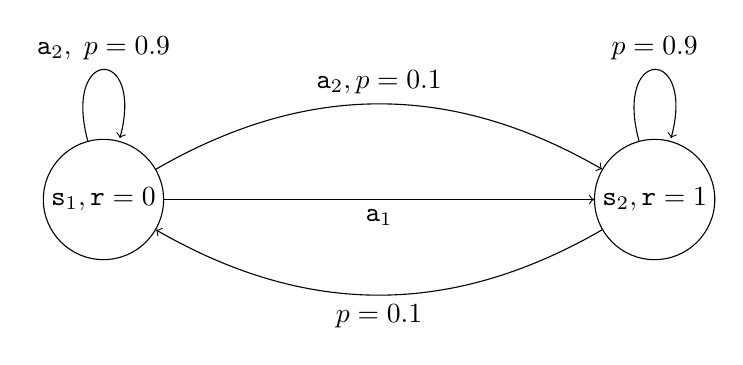
\begin{tikzpicture}[node distance=7cm, auto]
    % Nodes
    \node[draw, circle, inner sep=2pt] (S1) {\(\state_1, \reward=0\)};
    \node[draw, circle, inner sep=2pt, right of=S1] (S2) {\(\state_2, \reward=1\)};
    
    % Edges from S1
    \draw[->, bend left] (S1) to node[midway, above] {\(\action_2, p=0.1\)} (S2);
    \draw[->, right] (S1) to node[midway, below] {\(\action_1\)} (S2);
    \draw[->] (S1) edge[loop above] node {\(\action_2,\;p=0.9\)} (S1);
    
    % Edges from S2
    \draw[->] (S2) edge[loop above] node {\(p=0.9\)} (S2);
    \draw[->, bend left] (S2) to node[midway, below] {\(p=0.1\)} (S1);
\end{tikzpicture}
    \caption{Example MDP}
    \label{fig:vi_vs_pi_example}
\end{figure}
Let the policy in state \(\state_1\) be parametrized by $x$:
\[
x = \policy(\action_1), \quad \text{and hence} \quad \policy(\action_2) = 1-x.
\]
The corresponding Bellman equations for the value functions are:

\[
\begin{aligned}
\Value^\policy(\state_1) &= \gamma \Bigl[ x\,\Value^\policy(\state_2) + (1-x)\Bigl(0.1\,\Value^\policy(\state_2) + 0.9\,\Value^\policy(\state_1)\Bigr)\Bigr], \\
\Value^\policy(\state_2) &= 1 + \gamma \Bigl[0.9\,\Value^\policy(\state_2) + 0.1\,\Value^\policy(\state_1)\Bigr].
\end{aligned}
\]
Thus, substituting \(\gamma = 0.5\):
\[
\Value^\policy(\state_1) = 0.5 \Bigl[(0.9x+0.1)\Value^\policy(\state_2) + 0.9(1-x)\Value^\policy(\state_1)\Bigr].
\]
Rearranging, we obtain
\[
\Value^\policy(\state_1) = \frac{0.5(0.9x+0.1)}{0.55+0.45x}\,\Value^\policy(\state_2).
\]
Now, substitute into the \(\state_2\) equation to obtain:
\[
\Value^\policy(\state_2) = \frac{11+9x}{6+4.5x}, \quad
\Value^\policy(\state_1) = \frac{9x+1}{6+4.5x}.
\]
\textbf{Policy Iteration:} we compute PI iterates starting from a policy $\policy_0$ that chooses \(\action_2\) in \(\state_1\), i.e., \(x=0\). Thus,
\[
\begin{aligned}
\Value^{\policy_0}(\state_1) &= \frac{9\cdot 0 + 1}{6 + 4.5\cdot 0} = \frac{1}{6} \approx 0.16667,\\[1mm]
\Value^{\policy_0}(\state_2) &= \frac{11 + 9\cdot 0}{6 + 4.5\cdot 0} = \frac{11}{6} \approx 1.83333.
\end{aligned}
\]
Using the value function for \(\pi_0\), we compute the action-value functions in \(\state_1\):
\[
\begin{aligned}
\QValue^{\policy_0}(\state_1,\action_1) &= 0 + 0.5\,\Value^{\policy_0}(\state_2) \approx 0.5 \times 1.83333 = 0.91667,\\[1mm]
\QValue^{\policy_0}(\state_1,\action_2) &= 0 + 0.5\Bigl[0.1\,\Value^{\policy_0}(\state_2)+0.9\,\Value^{\policy_0}(\state_1)\Bigr] \\
           &\approx 0.5\Bigl[0.18333 + 0.15\Bigr] \approx 0.16667.
\end{aligned}
\]
Since \(\QValue^{\policy_0}(\state_1,\action_1) > \QValue^{\policy_0}(\state_1,\action_2)\), the improved policy \(\pi_1\) chooses \(\action_1\) (i.e., \(x=1\)). Then,
\[
\begin{aligned}
\Value^{\policy_1}(\state_1) &= \frac{9\cdot 1 + 1}{6 + 4.5\cdot 1} = \frac{10}{10.5} \approx 0.95238,\\[1mm]
\Value^{\policy_1}(\state_2) &= \frac{11 + 9\cdot 1}{6 + 4.5\cdot 1} = \frac{20}{10.5} \approx 1.90476.
\end{aligned}
\]
Policy $\policy_1$ is optimal, therefore PI will halt after one iteration. \\
\textbf{Value Iteration:}
the VI updates are as follows. 
\[
V_{k+1}(\state_1) = \max\Bigl\{ 0.5\,V_k(\state_2),\, 0.5\Bigl[0.1\,V_k(\state_2) + 0.9\,V_k(\state_1)\Bigr] \Bigr\},
\]
\[
V_{k+1}(\state_2) = 1 + 0.5\Bigl[0.9\,V_k(\state_2) + 0.1\,V_k(\state_1)\Bigr].
\]
\begin{figure}[ht]
    \centering
    \includegraphics[width=0.8\linewidth]{figures/vi_vs_pi.png}
    \caption{Comparison between VI and PI for the MDP in Figure \ref{fig:vi_vs_pi_example}. PI starts with a policy $x=0$, and VI is initialized with $V_0(\state_1) = 5, V_0(\state_2) = -1$.}
    \label{fig:vi_vs_pi_plot}
\end{figure}
In Figure \ref{fig:vi_vs_pi_plot} we illustrate the differences between the VI and PI algorithms for this MDP, by inspecting the values obtained during the algorithm runs. First, in the green line, we plot the values of all possible policies in this MDP (by varying $x$ in $[0,1]$). Note that the two policy iteration steps correspond to the two end points on this line. Next, we plot the VI iterates. We color in red the iterates for which the greedy policy (with respect to $V_k$) is optimal, while an orange color indicates otherwise. We make several important observations:
\begin{itemize}
    \item While the values of PI steps correspond to values of actual policies, the VI iterates $V_k$ do not necessarily correspond to any possible value functions (in the example, the VI iterates do not intersect the green line). Recall that we are only guaranteed that VI \textit{converges} to the value of an optimal policy. 
    \item Note that the greedy policy with respect to VI iterate converges to an optimal policy before the VI algorithm converged (in this case, already at $k=2$). Still, PI converges faster.
\end{itemize}
\end{example}
% \section{Variants on Value Iteration and Policy Iteration}

% \subsection{Value Iteration - Gauss Seidel Iteration}
% In the standard value iteration: ${\Value_{n + 1}} =
% T_{}^*({\Value_n})$, the vector ${\Value_n}$ is held fixed while all
% entries of ${\Value_{n + 1}}$ are updated. An alternative is to
% update each element ${\Value_n}(\state)$ of that vector as to
% ${\Value_{n + 1}}(\state)$ as soon as the latter is computed, and
% continue the calculation with the new value. This procedure is
% guaranteed to be ``as good'' as the standard one, in some sense, and
% often speeds up convergence.


% \subsection{Asynchronous Value  Iteration}
% Here, in each iteration ${\Value_n} \Rightarrow {\Value_{n + 1}}$,
% only a subset of the entries of  ${\Value_n}$ (namely, a subset of
% all states) is updated. It can be shown that if each state is
% updated infinitely often, then ${\Value_n} \to {\Value^*}$.
% Asynchronous update can be used to focus the computational effort on
% ``important'' parts of a large-state space.



% \subsection{Modified (a.k.a. Generalized or Optimistic) Policy Iteration}\label{ss:mod_PI}

% This scheme combines policy improvement steps with value iteration
% for policy evaluation. This way the requirement for exact policy
% evaluation (computing  ${\Value^{{\policy _k}}} = {(I - \discount
% {P^{{\policy _k}}})^{ - 1}}{r^{{\policy _k}}}$) is avoided.

% The procedure starts with some initial value vector ${\Value_0}$,
% and iterates as follows:
% \begin{itemize}
%   \item Greedy policy computation:

% Compute ${\policy _k} \in \arg {\max _\policy }T_{}^\policy
% ({\Value_k})$, a greedy policy with respect to ${\Value_k}$.
%   \item Partial fixed-point value iteration:

% Perform ${m_k}$ steps of value iteration, ${\Value_{k + 1}} =
% {(T_\discount ^{{\policy _k}})^{{m_k}}}({\Value_k})$.
% \end{itemize}

% This algorithm guarantees convergence of ${\Value_ k}$ to
% ${\Value^*}$.

%%%%%%%%%%%%%%%%%%%%%%%%%%%%%%%%%%%%%%%%%%


% \begin{leftbar}
% \section{Linear Program}
% \label{chapter-discount:section:LP}

% %[Good idea to add to get them familiar with the notion and notation for the very simple case.]



% %\section{Linear Programming for Finite Horizon}
% In this section we will use linear programming to derive the optimal
% policy for discounted return.
% %
% We will extend the linear programming given in Section
% \ref{C-MDP-FH:sec:LP} from Finite Horizon return to discounted
% return, but the derivation is similar in spirit.
% %
% %[YM: The preliminaries of the Linear Programming should move here
% %from Chapter of discounted return, if we keep this.]
% %
% We will see that both the primal and dual program will play an
% important part in defining the optimal policy. We will fix an
% initial state $\state_0$ and compute the optimal policy for it.

% We will start with the primal linear program, which will compute the
% optimal policy. For each state $\state$ and action $\action$ we will
% have a variable $x(\state,\action)$ that will indicate the
% discounted fraction of time we are at state $\state$ and perform
% action $\action$.

% To better understand what we mean by the ``discounted fraction of
% time'' consider a fixed policy $\policy$ and a trajectory
% $(\state_0, \ldots )$ generated by $\policy$. Define
% $X^\policy(\state,\action)=\sum_\ttime
% \I(\state_\ttime=\state,\action_\ttime=\action)$, which is a random
% variable. We are interested in
% $x^\policy(\state,\action)=\E[X^\policy(\state,\action)]$ which is
% the expected discounted fraction of time policy $\policy$ is in
% state $\state$ and performs action $\action$. The goal of our linear
% program is to compute $x^{\policy^*}$ for the optimal policy
% $\policy^*$.

% Our main constraint will be a flow constraint, stating that the
% discounted fraction of time we reach state $\state$ upper bounds the
% discounted fraction of time we exit it, times the discounted factor.
% Formally, for $\state\in\States$,
% \[
% \I(\state=\state_0)+\sum_{\action} x(\state,\action)\leq \discount
% \sum_{\state',\action'}
% x(\state',\action')\transitionprob(\state|\state'\action').
% \]
% Note that if we sum the inequalities over all states, we have
% \[
% 1+\sum_{\state,\action} x(\state,\action)\leq\discount
% \sum_{\state',\action'} x(\state',\action')\sum_\state
% \transitionprob(\state|\state'\action')=\discount \sum_{\state',\action'}
% x(\state',\action').\]
% %
% which implies that $\sum_{\state,\action} x(\state,\action)\leq
% 1/(1-\discount)$, as we should expect. Namely, in each time we are
% in some state, therefore the sum over states should be $\sum_\ttime
% \discount^\ttime=1/(1-\discount)$.

% The discounted return, which we would like to maximize, is
% $\E[\sum_\ttime
% \discount^\ttime\reward(\state_\ttime,\action_\ttime) ]$. We can
% regroup the sum by state and action and have
% $\sum_{\state,\action}\E[\sum_\ttime
% \discount^\ttime\reward(\state_\ttime,\action_\ttime)\I(\state_\ttime=\state,\action_\ttime=\action)]$,
% which is equivalent to $\sum_{\state,\action}\reward(\state,\action)
% \E[\sum_\ttime
% \discount^\ttime\I(\state_\ttime=\state,\action_\ttime=\action)]$.
% Now our variable are $x(\state,\action)=\E[\sum_\ttime
% \discount^\ttime\I(\state_\ttime=\state,\action_\ttime=\action)]$,
% and the expected return would be
% \[
% \sum_{\state,\action} \reward(\state,\action)x(\state,\action)
% \]


% The resulting linear program is the following.

% \begin{align*}
% \max_{x(\state,\action)}&\;\;\; \sum_{\state,\action}
% \reward(\state,\action)x(\state,\action)\\
% &\mbox{ such that }\\
% %
% &\I(\state=\state_0)+\sum_{\action} x(\state,\action)\leq \discount
% \sum_{\state',\action'} x(\state',\action')\transitionprob(\state|\state'\action')
% &\quad\forall \state \in {\States}, \action\in\Actions,\\
% %
% % &\sum_{\action}
% %x_{\ttime}(\state,\action)=\sum_{\state',\action'}
% %x_{\ttime-1}(\state',\action')p_{\ttime-1}(\state|\state'\action').
% % &\quad\forall
% %\state \in {\States_{\ttime}}, \action\in\Actions,
% %\ttime\in\T\\
% %
% &x(\state,\action) \geq 0  &\quad\forall \state \in {\States},
% \action\in\Actions,
% \\
% %
% %&x_{\ttime}(\state,\action) \leq 1   &\quad\forall \state \in
% %{\States_{\ttime}}, \action\in\Actions,
% %\ttime\in\{0,\ldots,\tHorizon-1\}\\
% %
% &\sum_{\action}x_{0}(\state_0,\action)=1 &\quad\forall \action\in\Actions,\\
% &x_{0}(\state,\action)=0,  &\quad\forall \state \in {\States},
% \state\neq \state_0\\
% \end{align*}

% Given the primal linear program we can derive the dual linear
% program.
% \begin{align*}
% \min_{z(\state)}  \;z_0(\state_0)&\\
% \mbox{ such that }\\
% %
%  z(\state) &\geq
% \reward(\state,\action) + \discount
% \sum_{\state'}z(\state')\transitionprob(\state'|\state,\action) , &\quad\forall
% \state \in {\States},\action\in\Actions, \\ .
% \end{align*}

% One can identify the dual random variables $z(\state)$ with the
% optimal vale function $\Value(\state)$. At the optimal solution of
% the dual linear program one can show that we have
% \begin{align*}
%  z(\state) &= \max_\action \big\{
% \reward(\state,\action) + \discount
% \sum_{\state'}z(\state')p_{\ttime}(\state'|\state,\action) \big\} ,
% &\quad\forall \state \in {\States},
% \end{align*}
% which are the familiar Bellman optimality equations.

% %
% %
% %\begin{proposition}
% %The solution $v_\ttime(\state)$ of the linear program is the optimal
% %value function $\Value_{ttime}(\state)$.
% %\end{proposition}
% %
% %\begin{proof}
% %Let $v_\ttime(\state)$ be the solution of the linear program. We
% %will show by back ward induction that the values $v_\ttime(\state)$
% %are identical to $\Value_\ttime(\state)$ of the Finite-horizon
% %Dynamic Programming (Algorithm \ref{Alg:FHDP-DDP}), i.e,
% %$v_\ttime(\state)=\Value_\ttime(\state)$.
% %
% %At $\ttime=\tHorizon$ it holds by the initializations in both cases.
% %Consider $\ttime$ and assume that the inductive hypothesis holds for
% %$\ttime+1$. This implies that for every action $\action\in\Actions$
% %nd state $\state\in\States$, we have
% %\[{{\reward_{\ttime}}(\state,\action) + \Value_{\ttime +
% %1}^{}({f_{\ttime}}(\state,\action))}=
% %{{\reward_{\ttime}}(\state,\action) + v_{\ttime +
% %1}^{}({f_{\ttime}}(\state,\action))} .\]
% %Therefore we have
% %$v_\ttime(\state) \geq \Value_\ttime(\state)$. Since we are
% %minimizing over $v_\ttime(\state)$, we have $v_\ttime(\state) \geq
% %\Value_\ttime(\state)$.
% %\end{proof}

% \end{leftbar}

% \section{Exercises}
% \subsection{Modified Policy Iteration:}
In this question we will analyze the Modified Policy Iteration (MPI) algorithm~\ref{alg:MPI}. 
% Denote the fixed-policy and optimal Bellman operators as $T^\pi$ and $T$, respectively. 
\begin{center}
\begin{minipage}{1.1\textwidth}
\begin{algorithm}[H]
	\caption{MPI}
	\label{alg:MPI}
	\begin{algorithmic}
		\STATE {\bfseries Initialize:} $m \in \mathbb{N},~\Value_0 \in \mathbb{R}^{|\States|}$
		\WHILE{some stopping criterion}
			\FOR{ $\state\in \States$}
				\STATE $\policy_{k+1}(\state)\in \arg\max_{\action} \reward(\state,\action) + \gamma \sum_{\state'}\transitionprob(\state' | \state,\action)\Value_k(\state').$
			\ENDFOR
			\FOR{$\state\in \States$}
				\STATE $\Value_{k+1}(\state)= \sum_{\ttime=0}^{m-1}\sum_{\state'} \gamma^\ttime \transitionprob(\state_\ttime=\state' | \state_0=\state,\policy_{k+1}) \reward(\state',\policy_{k+1}(\state')) +\gamma^m \sum_{\state''}\transitionprob(\state_m=\state'' | \state_0=\state, \policy_{k+1})\Value_{k}(\state'').$
			\ENDFOR
		\ENDWHILE
		\STATE {\bfseries Return $\policy,\Value$}
	\end{algorithmic}
\end{algorithm}
\end{minipage}
\end{center}

\begin{itemize}
\item [a.] In a vector notation, MPI performs the following two steps of policy and value update,
\begin{enumerate}
\item $\policy_{k+1} \in \{\policy': T^{\policy'}\Value_k=T \Value_k \}$.
\item $\Value_{k+1} =\left(T^{\policy_{k+1}}\right)^m \Value_{k}$.
\end{enumerate}
Prove the two algorithms are equivalent.
\item [b.] Describe which algorithms are obtained when $m=1,m\to\infty$? 
\end{itemize}

In the rest of the question we will analyze the convergence of Modified Policy Iteration.
\begin{itemize}
\item [c.] Assume that $T \Value_0\geq \Value_0$. Prove the following (component-wise) inequalities $$\Value_0\leq T^{\policy_1} \Value_0 \leq \cdot\cdot\cdot \leq (T^{\policy_1})^m \Value_0\leq (T^{\policy_1})^{m+1} \Value_0 \leq \cdot \cdot \cdot \leq \Value^{\policy_1} \leq \Value^*.$$
Do the inequalities hold without the assumption? prove or give a counter-example.
\item [d.] Assume that $T \Value_0\geq \Value_0$. Prove that for any $k$, $T \Value_k\geq \Value_k$ (component-wise) and thus $$\Value_{k-1}\leq T^{\policy_k}\Value_{k-1} \leq \cdot\cdot\cdot \leq (T^{\policy_k})^m \Value_{k-1} \leq (T^{\policy_k})^{m+1} \Value_{k-1}\leq \cdot \cdot \cdot \leq \Value_{\policy_{k}}\leq \Value_*$$ for any $k$.
Hint: use induction, and the update rule of MPI, $\Value_k=(T^{\policy_k})^m \Value_{k-1}$.
\item [e.] Prove $\norm{\Value_*-\Value_k}_\infty \leq \gamma \norm{\Value_*-\Value_{k-1}}_\infty$. Hint: prove $0 \leq \Value_*-\Value_k\leq T\Value_* - T\Value_{k-1}$ and then take the max-norm.
\end{itemize}
% \subsection{MDP with a reward-ratio objective:}
Consider an MDP $\mathcal{M}$ with finite state space $\mathcal{S}$ and finite actions space $\mathcal{A}$, transitions $P(s'|s,a)$, discount factor $\gamma\in (0,1)$, a \textbf{fixed} initial state $s_{init}$, and \textbf{two} reward functions: $r_1(s)$ and $r_2(s)$. In this question we will consider objectives that are a function of both $r_1$ and $r_2$.

For a Markov policy $\pi$, we denote the discounted returns $J_1^\pi$ and $J_2^\pi$ as:
\begin{equation*}
\begin{split}
    J_1^\pi &= \mathbb{E}^\pi \left[\left. \sum_{t=0}^\infty \gamma^t r_1(s_t)\right|s_0 = s_{init}\right], \\
    J_2^\pi &= \mathbb{E}^\pi \left[ \left.\sum_{t=0}^\infty \gamma^t r_2(s_t)\right|s_0 = s_{init}\right].
\end{split}
\end{equation*}

Note that the initial state is fixed, and that $J_1^\pi, J_2^\pi$ denote scalar returns and not value functions.

Let $f(x,y)$ be some function of two variables. For some policy $\pi$ we denote $J^\pi = f(J_1^\pi, J_2^\pi).$ We wish to find a policy $\pi^*$ that maximizes $J^\pi$:
\begin{equation*}
    J^* = \max_{\pi} J^\pi, \quad \pi^* \in \argmax_{\pi} J^\pi.
\end{equation*}

\begin{itemize}
    \item[a.] For $f(x,y)=\alpha x +\beta y$, propose a standard MDP with a single reward $\hat{r}$ such that it's optimal policy is $\pi^*$. Explain.
\end{itemize}

For the rest of this question, we consider the function $f(x,y) = \frac{x}{y}$. Furthermore, we assume the following bounds on the rewards: $0<r_{min}\leq r_1(s) < r_2(s) \leq r_{max}$, for all $s\in\mathcal{S}$. 

\begin{itemize}
    \item[b.] Can the standard MDP solution approaches (value iteration, policy iteration) be used to find $\pi^*$ in this case? Explain (no need to prove formally).
\end{itemize}

For some $\rho \in [0,1]$, consider a standard MDP $\mathcal{M}_{\rho}$ with the same $\mathcal{S},\mathcal{A},P,\gamma$ as $\mathcal{M}$ and reward $\hat{r}(s) = r_1(s) - \rho r_2(s).$ Denote the discounted reward for a policy $\pi$ in $\mathcal{M}_{\rho}$ as $J_{\rho}^\pi = \mathbb{E}^\pi \left[ \sum_{t=0}^\infty \gamma^t \hat{r}(s_t)|s_0 = s_{init}\right]$.

\begin{itemize}
    \item[c.] Assume that for some policy $\pi$, we have that $J_{\rho}^\pi = 0$. What is $J^\pi$?
    \item[d.] Let $\pi_\rho^*$ be an optimal policy in $\mathcal{M}_{\rho}$, that also satisfies  $J_{\rho}^{\pi_\rho^*} = 0$. Show that $\pi_\rho^*$ is optimal also in $\mathcal{M}$.
    
    Hint: assume that for some $\pi'$, $J^{\pi'} > \rho$, and show a contradiction.
    
    \item[e.] Show that for $\rho=0$, $J_{\rho}^\pi > 0$ for any $\pi$.
    \item[f.] Show that for $\rho=1$, $J_{\rho}^\pi < 0$ for any $\pi$.
    \item[g.] Let $J_{\rho}^*$ denote the optimal value in $\mathcal{M}_{\rho}$. Show that $J_{\rho}^*$ is monotonically decreasing in $\rho$.
    
    Hint: start by showing monotonicity for a fixed policy.
    \item[h.] Based on (d-g), propose an approach for finding the optimal policy $\pi^*$. Technically, you can assume that $J_{\rho}^*$ is continuous in $\rho$, and you can invoke any standard MDP solver in your solution.
    
\end{itemize}
% \subsection{Purchasing with a deadline}
Consider the following scenario: as the purchasing manager of a factory, you have $T$ days to buy a certain material that is required for the production process. At the beginning of each day $k$, you observe a price offer for the material $x_k \sim \mathit{Uniform}[a,b]$, drawn independently of the prices at other days. You may decide to either buy the material at the price $x_k$ (and then the scenario ends), or wait for the next day. If a purchase hasn't been made by day $T$, the product has to be purchased at the last price $x_T$.

The goal is to decide when to buy the material, such that its price (in expectation) is lowest.

1. Explain intuitively, why the optimal decision whether to buy at some price $x$ may be different at different days.

We formulate the problem as a finite horizon MDP as follows. The state space at time $k$ is $x_k\in [a,b]$. The action space is binary $a_k \in \{buy,hold\}$. Once a $buy$ action is executed at state $x_k$, an immediate cost of $x_k$ is incurred, and the state transitions to a terminal state $x^*$ with zero cost. Otherwise, if a   $hold$ action is executed, no cost is incurred, and the state transitions to $x_{k+1} \sim \mathit{Uniform}[a,b]$. At time $k=T$, the only available action is $buy$. Also, once the terminal state is reached, the state no longer changes, and no cost is further incurred.

2. Define the optimal value function $V_k(x) \doteq \inf_\pi \mathbb{E}^\pi \left[ \sum_{t=k}^{T} c(x_t,\pi(x_t)) | x_k = x\right]$. Note that by definition $V_k(x^*)=0$ for all $k$.

%\quad a. What is $V_k(x^*)$?

\quad a. What is $V_T(x)$?

\quad b. Write a recursive equation for $V_k(x)$ as a function of  $V_{k+1}(x)$.

3. For $a=0,b=1$, draw the value functions $V_T(x)$, $V_{T-1}(x)$, and $V_{T-2}(x)$.

4. Prove that the optimal policy is a threshold policy, given by
\begin{equation*}
\left\{
  \begin{array}{ll}
    buy, & \text{if } x_k \leq \alpha_k \\
    hold, & \text{if } x_k > \alpha_k.
  \end{array}
\right.
\end{equation*}

\quad Write a recursive equation for $\alpha_k$.

\vspace{20pt}
From now on, we consider a scenario where there is correlation between the prices at different days. Specifically:
\begin{equation*}
    x_{k+1} = \lambda x_k + \epsilon_k,
\end{equation*}
where $0 \leq \lambda < 1$ is a known constant, and $\{\epsilon_k\} \in [0,b]$ are i.i.d. random variables with a known distribution $p(\epsilon)$. Let $\bar{\epsilon} = \mathbb{E} [\epsilon_k ]$, and assume that $\bar{\epsilon} > 0$. The state space in this case is $x_k\in \mathbb{R}$.

5. Write a recursive equation for the value function $V_k(x)$ for this scenario.

\vspace{10pt}

We will now show that in the correlated case as well, the optimal policy is a threshold policy. We will do this in several steps.

A function $f(x)$ is said to be \emph{concave} if, for any $x,y$ and $\beta \in [0,1]$, it holds that $f(\beta x + (1-\beta) y) \geq  \beta f(x) + (1-\beta) f(y)$.

6. Prove that if $f(x)$ is concave, then $\mathbb{E} [f(\lambda x + \epsilon_k)]$ is also concave.

7. Prove that for all $1 \leq k \leq T$, the value function $V_k(x)$ is concave.

\quad \textbf{Hint}: you may use the following fact: the minimum of two concave functions is concave.

%A function $f(x)$ is said to be \emph{increasing} if, for any $x<y$ it holds that $f(x) < f(y)$.

8. * Prove that the optimal policy is again a threshold policy.

\quad \textbf{Hint}: You may first prove that for all $1 \leq k \leq T$, $V_k(x)$ is increasing, and positive for $x\geq 0$. 

\section{Further Remarks on Policy Iteration}
\label{disc:bib}

% The value iteration method dates back  to Bellman \cite{Bellman:DynamicProgramming}.
% The computational complexity analysis of value iteration first explicitly appeared in \cite{LittmanDK95}.
%
% The work of Blackwell \cite{blackwell1965discounted} introduces the contracting operators and the fixed point for the analysis of MDPs.

Policy iteration originated in the work of Howard \cite{Howard1960}.
There has been significant interest in bounding the number of iteration of policy iterations, with a dependency only on the number of states and actions. A simple upper bound is the number of policies, $|\Actions|^{|\States|}$, since each policy is selected at most once.
The work of \cite{MelekopoglouC94} shows a lower bound of $\Omega(2^{|\States|/2})$ for a special class of policy iteration, where only a single state of all improving states is updated and two actions.
The work of \cite{MansourS99} shows that if the policy iteration updates with all the improving states (as it is define here) then the number of iterations is at most $O(|\Actions|^{|\States|}/|\States|)$.
The work of \cite{Fearnley10} shows a $n$-state and $\Theta(n)$ action MDP for which the policy iteration requires $\Omega(2^{n/7})$ iterations for the average cost return, and \cite{HollandersDJ12} for the discounted return. Surprisingly, for a constant discount factor, the bound on the number of iterations is polynomial \cite{Ye11,HansenMZ13}.




%The work of \cite{d1963probabilistic} was the first to formalize a Linear Programming for the discounted return, and \cite{manne1960linear} for the average cost.
%There are works that use a linear programming approach to derive strongly polynomial algorithms. Specifically, for deterministic MDPs we have polynomial time algorithms which are based on linear programming \cite{MadaniTZ10,PostY13}.

\bibliographystyle{plain}
\bibliography{bib-lecture}
\end{document}
